\documentclass[conf]{new-aiaa}
\usepackage[utf8]{inputenc}

\usepackage{graphicx}
\usepackage{amsmath}
\usepackage[version=4]{mhchem}
\usepackage{siunitx}
\usepackage{longtable,tabularx}
\setlength\LTleft{0pt}
\usepackage{cleveref}
\usepackage{booktabs}
\usepackage{mathtools}
\DeclarePairedDelimiter{\abs}{\lvert}{\rvert}
\usepackage{subfig}
\usepackage{float}

\title{Takeoff and Performance Tradeoffs of Retrofit Distributed Electric Propulsion for Urban Transport}

\author{\
Kevin R. Moore\footnote{Masters Student, Department of Mechanical Engineering, AIAA Student Member}
\ and Andrew Ning\footnote{Assistant Professor, Department of Mechanical Engineering, AIAA Senior Member}\\
{\normalsize\itshape
Brigham Young University, Provo, UT, 84602, USA}\
\\
\
{
}
}

\begin{document}

\maketitle

\begin{abstract}
    While vertical takeoff and landing aircraft have shown promise for urban air transport, distributed electric propulsion on existing aircraft may offer immediately implementable alternatives. Distributed electric propulsion could potentially decrease takeoff distances enough to enable thousands of potential inter-city runways. This conceptual study explores the effects of a retrofit of open-bladed electric propulsion units. To model and explore the design space we use blade element momentum method, vortex lattice method, linear-beam finite element analysis, classical laminate theory, composite failure, empirically-based blade noise modeling, motor and motor-controller mass models, and gradient-based optimization. With liftoff time of seconds and the safe total field length for this aircraft type undefined, we focused on the minimum conceptual takeoff distance. We found that 16 propellers could reduce the takeoff distance by over 50\% compared to the optimal 2 propeller case. This resulted in a conceptual minimum takeoff distance of 20.5 meters to clear a 50 ft (15.24 m) obstacle. We also found that when decreasing the allowable noise by approximately 10 dBa, the 8 propeller case performed the best with a 43\% reduction in takeoff distance compared to the optimal 2 propeller case. This resulted in a noise-restricted conceptual minimum takeoff distance of 95 meters.

\end{abstract}

\section{Introduction}
\label{chp:chapter1}
\graphicspath{{figures/}}

In early aircraft designs, distributed propulsion was used more out of necessity than deliberate choice. Designs such as the Dornier Do X in 1929, the Hughes H-4 Hercules in 1947, and many other large aircraft before the jet age, were constrained by the available propulsion units of the time~\cite{Gohardani:2011aa}. With the dawn of the jet age, aircraft began to use fewer but larger engines. However, some distributed and blended wing jet concepts were explored as early as 1954~\cite{dist_jet}. During the push for high altitude long endurance (HALE) aircraft design, distributed electric propulsion (DEP) emerged as a viable option with NASA's Pathfinder in 1983~\cite{Flittie:1998aa}. In 1988, NASA produced several concepts including distributed propulsion with the intention of lift augmentation~\cite{nasa_many_distrib}, which evolved until the Helios' destruction in 2003~\cite{Helios}. In the 2000s, a third wave of aeronautics began to emerge, termed by NASA as on demand mobility (ODM)~\cite{Moore:2006aa}, or unscheduled aircraft services. Within ODM, two applications have begun to be targeted: thin-haul commuters and urban air taxis~\cite{Hwang:2018aa}.

\begin{figure}[htbp]
    \centering
    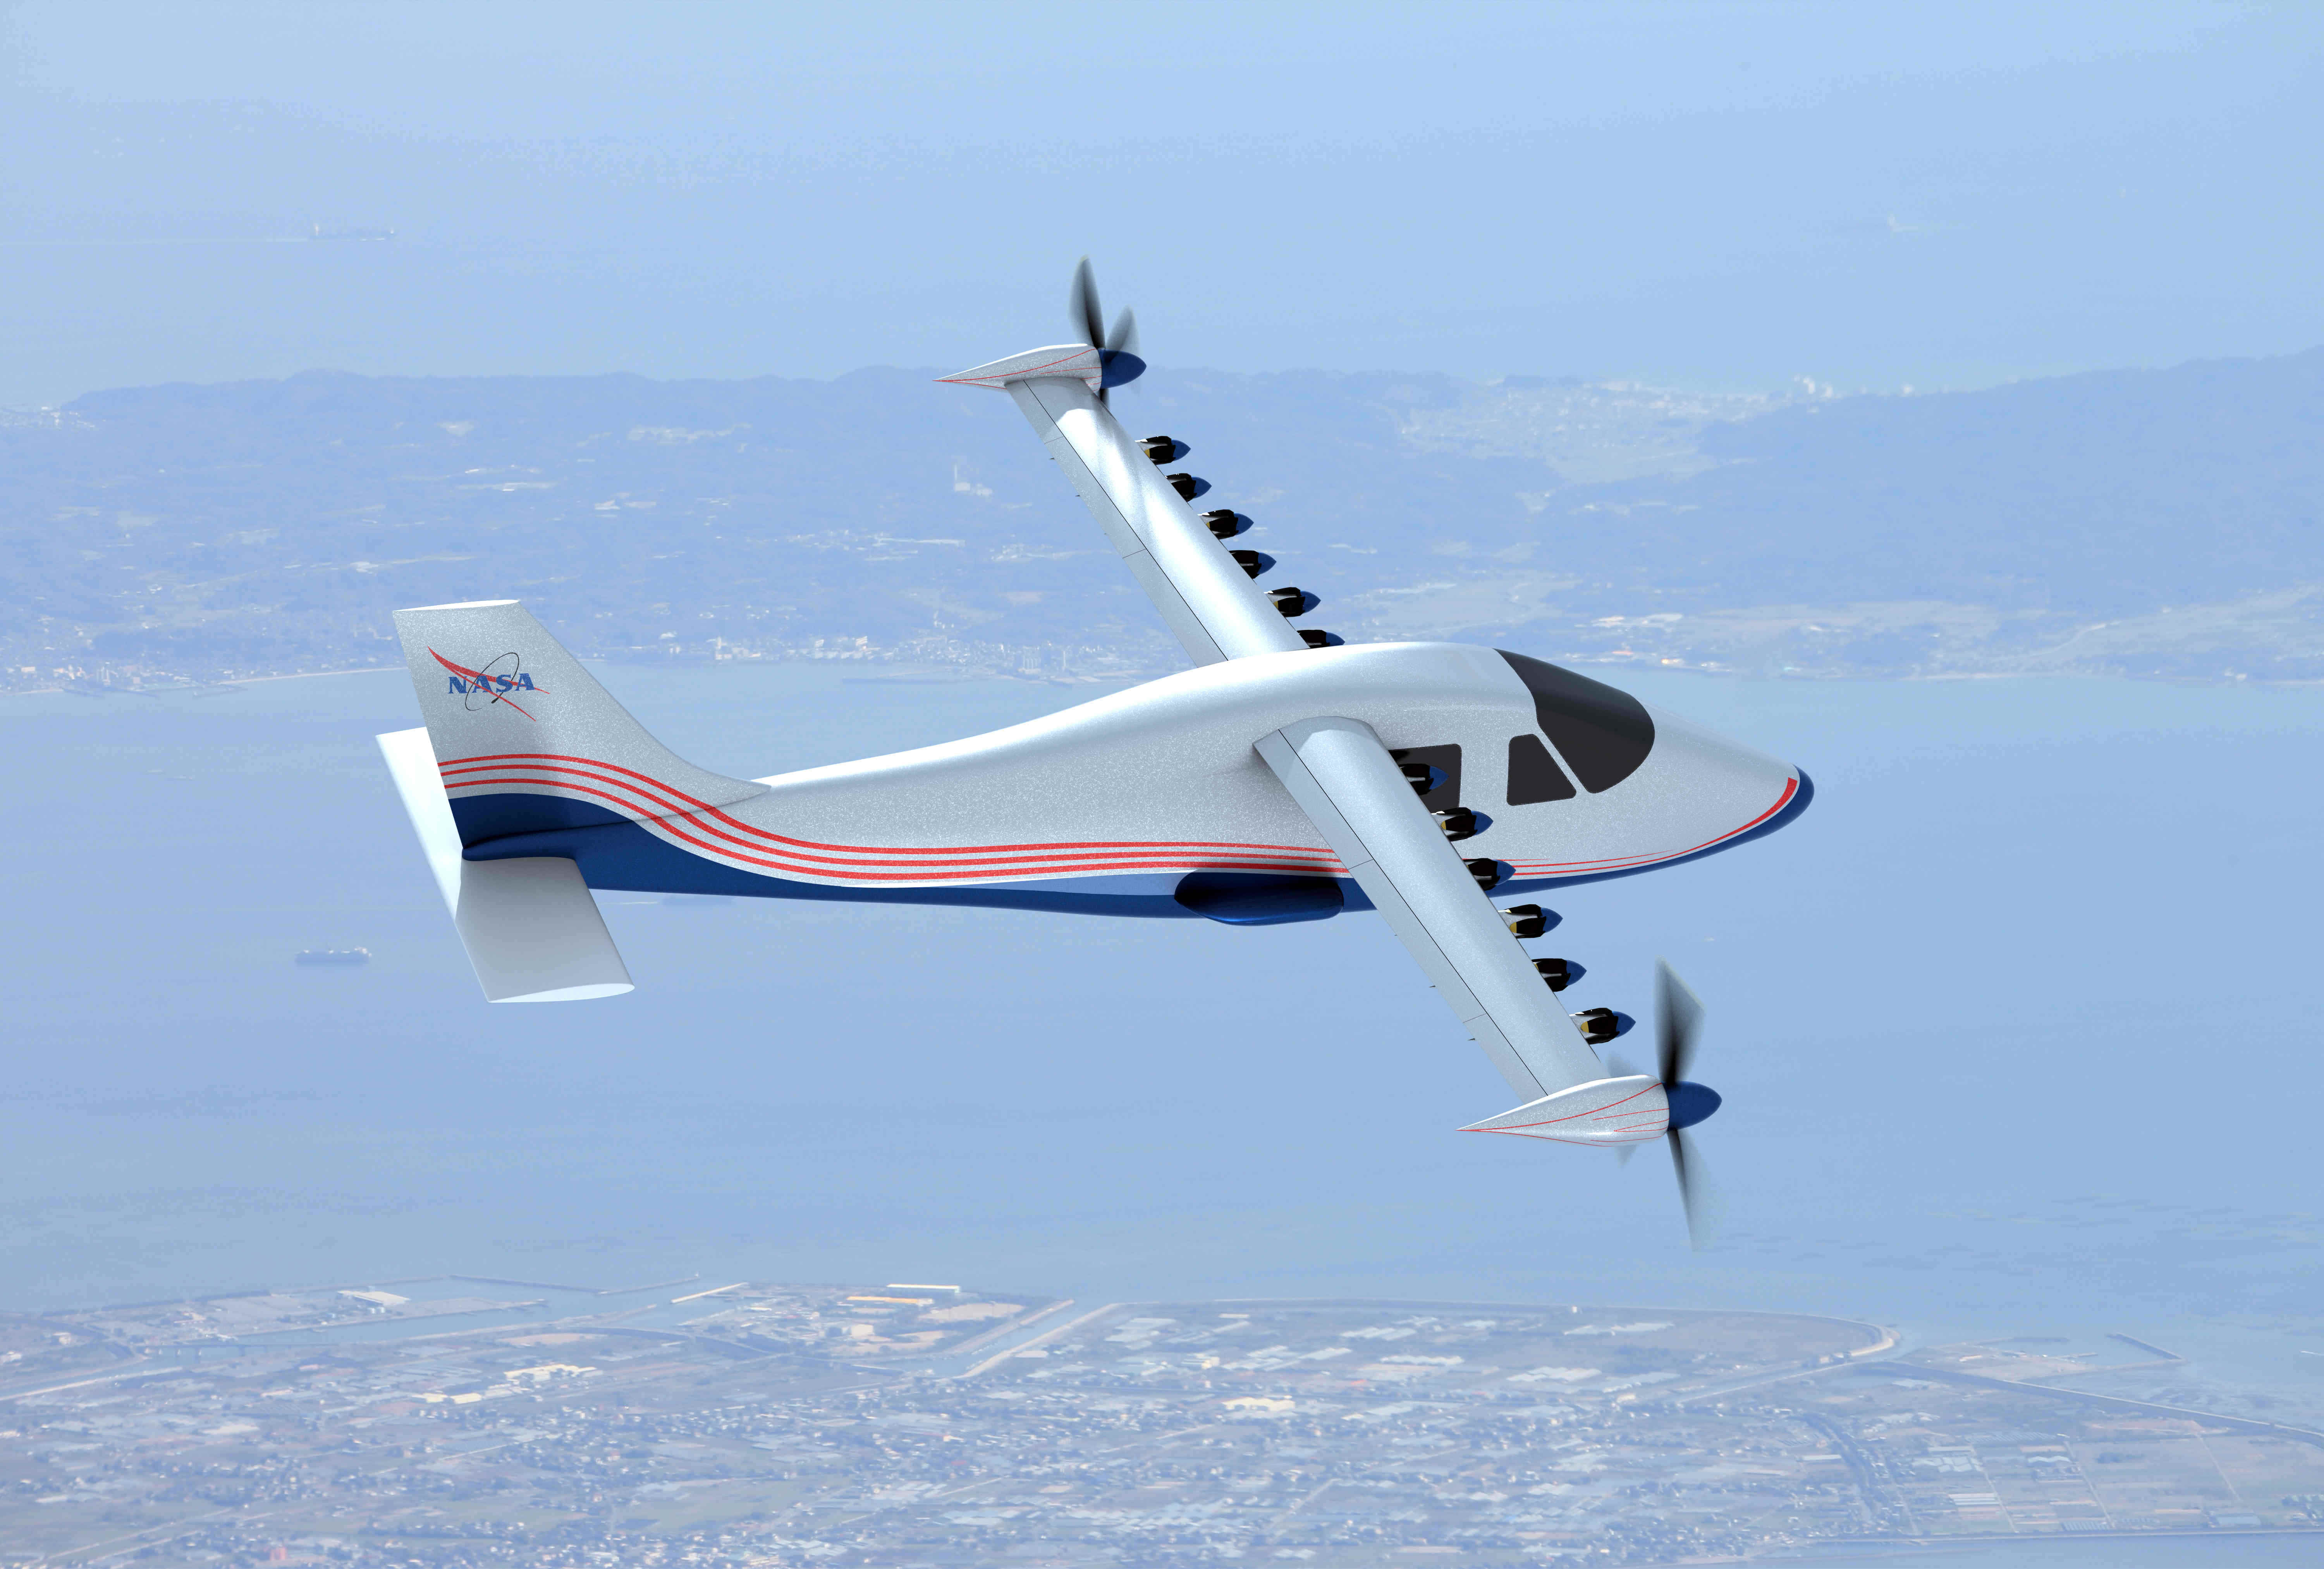
\includegraphics[trim={3.5cm 6.0cm 4.0cm 4.5cm},clip,width=3.0in]{leaptech}
    \caption[NASA X-57 thin-haul concept aircraft illustration showing the mid span DEP propellers in the folded cruise position.]{NASA X-57 thin-haul concept aircraft illustration\footnotemark~showing the mid span DEP propellers in the folded cruise position.}
    \label{f:leaptech1}
\end{figure}

\footnotetext{Image reprinted from ``NASA Electric Research Plane Gets X Number, New Name", by A. Beutel, 2017, Retrieved from https://www.nasa.gov/press-release/nasa-electric-research-plane-gets-x-number-new-name. Public Domain Credit: NASA}

Thin-haul commuters, the first ODM application, are aircraft designed to fly routes not justifiable by large airlines. An example concept emerged in 2014 when NASA partnered with Joby Aviation and Empirical Systems Aerospace to use the Leading Edge Asynchronous Propeller Technology (LEAPTech) as a test bed for distributed propulsion research~\cite{Stoll:2014aa}. Additionally, in 2016, NASA announced the X-57 Maxwell short haul commuter (see~\cref{f:leaptech1}) with goals to reduce the energy required for cruise by 4.8x without sacrificing cruise speed or takeoff distance~\cite{Borer:2017aa}. Since the X-57, there has been a significant increase in the amount of research regarding DEP for thin-haul commuters in areas such as economics\cite{Harish:2016aa}, multidisciplinary modeling requirements~\cite{Patterson:2014aa}, wing aerodynamic analysis~\cite{Deere:2017aa, Borer:2017aa, Stoll:2014aa}, motor design~\cite{Dubois:2016aa}, avionics~\cite{Clarke:2017aa}, hybrid propulsion~\cite{Papathakis:2018aa}, trajectory thermal considerations~\cite{Falck:2017aa}, certification and landing safety~\cite{Patterson:2017aa} and large scale multidisciplinary optimization of design and trajectory~\cite{Hwang:2018aa}.

Urban air taxis, the second ODM application, are aircraft designed for 2-6 passengers and distances less than 100 miles~\cite{Holmes:2016aa}. Though there is significant infrastructure required to adopt this type of transportation, there is potential for competitive operating costs~\cite{Antcliff:2016aa}. The economic possibilities have driven the development of a variety of concepts including tilt rotor, multi-rotor, and tilting ducted fans. The concept of urban air transport with conventional small fixed-wing aircraft as opposed to vertical takeoff and landing aircraft has been previously explored~\cite{Holmes:2004aa}. However, the concept of using distributed electric propulsion to shorten the runway distance is relatively recent. In the predecessor to this work~\cite{Moore:2018aa}, we used a propeller-on-wing aerodynamic model and electric component performance modeling to show an 80\% reduction in takeoff rolling distance using an optimal distributed electric propulsion design as opposed to an optimal two-propeller electric configuration. More recently, Courtin et al.~\cite{Courtin:2018aa} conducted a feasibility analysis of the STOL concept for urban air transport with the geometric programming (GP) method. They took a broad approach to the STOL urban air transport problem including takeoff rolling distance, landing distance, wing spar sizing using root bending moment, propulsion effects via 2D jets, and lift augmentation using a momentum balance. According to the study, runway lengths need only be less than 150 m (500 ft) to have feasible DEP aircraft access to thousands of potential locations in cities such as Dallas and Chicago.

This work builds upon previous work with the following contributions: First, we integrate a wide range of multidisciplinary models and constraints including propeller aerostructural coupling, propeller noise, aircraft takeoff path dynamics, propeller on wing interactions, power conversion efficiency, and electrical component mass. Second, we include model modifications that allow for efficient gradient based optimization using a new method for smooth gradients with respect to propeller on wing interactions. Third, we present several case studies looking at the sensitivity to a few critical parameters that help better understand the design tradeoffs of a short takeoff fixed wing aircraft in urban transport applications.

%%%%%%%%%%%%%%%%%%%%
%%  END INTRO
%%  START METHODOLOGY
%%%%%%%%%%%%%%%%%%%%

\section{Model Description}

In this section, models relating to propeller and wing aerodynamics, propeller noise, propeller aerostructural, and electrical component modeling are outlined. These include blade element momentum theory, airfoil preprocessing, BPM (Brooks, Pope, and Marcolini) noise modeling, composite structures, vortex lattice method, propeller on wing interaction modeling, electric motor performance and mass, motor controller mass, and battery mass. Several verification and validation cases are also presented.

\subsection{Propeller Aerodynamics}


We use CCBlade, an open source blade element momentum (BEM) code formulated to give guaranteed convergence and in turn allow for a continuously differentiable output~\cite{ccblade}.\footnote{CCBlade.jl on BYU FLOW Lab GitHub \href{https://github.com/byuflowlab/CCBlade.jl}{https://github.com/byuflowlab/CCBlade.jl}} It includes a non-normal inflow correction which allows us to mount the props in line with the wing and include the angle of attack (AOA) of the wing as the inflow angle to the prop. For atmospheric properties we use NASA's 1976 Standard Atmosphere Model\footnote{BYU FLOW Lab GitHub Atmosphere.jl \href{https://github.com/byuflowlab/Atmosphere.jl}{https://github.com/byuflowlab/Atmosphere.jl}}~\cite{Atmosphere:2014aa}. From CCBlade we extract axial and tangential induced flow distributions to be able to compute the propeller wake influence on the wing. This BEM formulation uses 2D airfoil data to calculate the induction factors for each annular disk of the propeller including Prandtl hub and tip loss correction factors~\cite{tip-correction}. To properly model the induced wake velocity in BEM formulation, the tip loss factors must be included in the output induced velocities.

Propeller wakes generally reach their far-field values within approximately one rotor radius~\cite{Alvarez:2018aa}. In this conceptual design study, we model the propeller as being removed one radius or more from the wing for the far-field values to be applied on the wing. This removes the need to model slipstream contraction and the associated changes in wing angle of attack and spanwise flow that would otherwise be present with a propeller closer than one radius to the wing. This configuration is similar to tests conducted by Veldhuis and Epema~\cite{proponwing, epema}. Additionally, in their experimental results, not all of the tangentially induced velocity from the propeller is applied normal to the wing chordline. This swirl reduction factor (SRF) is approximately 0.5~\cite{proponwing} for a propeller in line with the wing chord. Similar to that done by Veldhuis~\cite{proponwing}, we model the annular contraction as being fixed at the wake center with the contraction compounding to the edge of the stream tube. Applying the fully developed wake on the wing has the advantage of removing the need to model changes in the wing angle of attack due to wake contraction.

\subsubsection{Airfoil Pre-computation}


Blade element momentum theory is dependent on accurate airfoil data for accurate propeller performance prediction. To calculate the airfoil data, we use XFOIL\footnote{Xfoil.jl on BYU FLOW Lab GitHub \href{https://github.com/byuflowlab/Xfoil.jl}{https://github.com/byuflowlab/Xfoil.jl}} to run the Eppler 212 airfoil for thirteen Reynolds numbers ranging from $5 \times 10^4$ to $1 \times 10^8$, five Mach numbers ranging from 0 to 0.8, and fifty-one angles of attack ranging between negative and positive stall (approximately negative 10$^\circ$ to positive 20$^\circ$, depending on the Reynolds and Mach number).

We use Airfoilpreppy\footnote{AirfoilPreppy on BYU FLOW Lab GitHub \href{https://github.com/byuflowlab/AirfoilPreppy}{https://github.com/byuflowlab/AirfoilPreppy}}~\cite{airfoilpreppy} to model the stall delay experienced by local sections on rotating blades. This code applies the rotational correction on lift by Du et al.~\cite{Du:1998aa} and drag by Eggers et al.~\cite{Eggers:2003aa} as well as extrapolation to high angles of attack by Viterna et al.~\cite{Viterna:1982aa}.

\subsubsection{Propeller Performance Comparison}

\label{PropPerformance}

To validate that the BEM code with XFOIL airfoil data calculation was consistent with Epema's published experimental cases~\cite{epema}, we compared his published experimental results with our computational model of his setup. The results for a constant RPM and varying freestream are seen in~\cref{fig:eta_prop}. Since the 2D airfoil data includes stall, the modeled effects of stall can be seen on the 3D propeller performance for very low advance ratios. The more linear regions at the lowest advance ratios are comprised of post-stall angles of attack calculated by the Viterna extrapolation.

\begin{figure}[htbp]
    \centering
    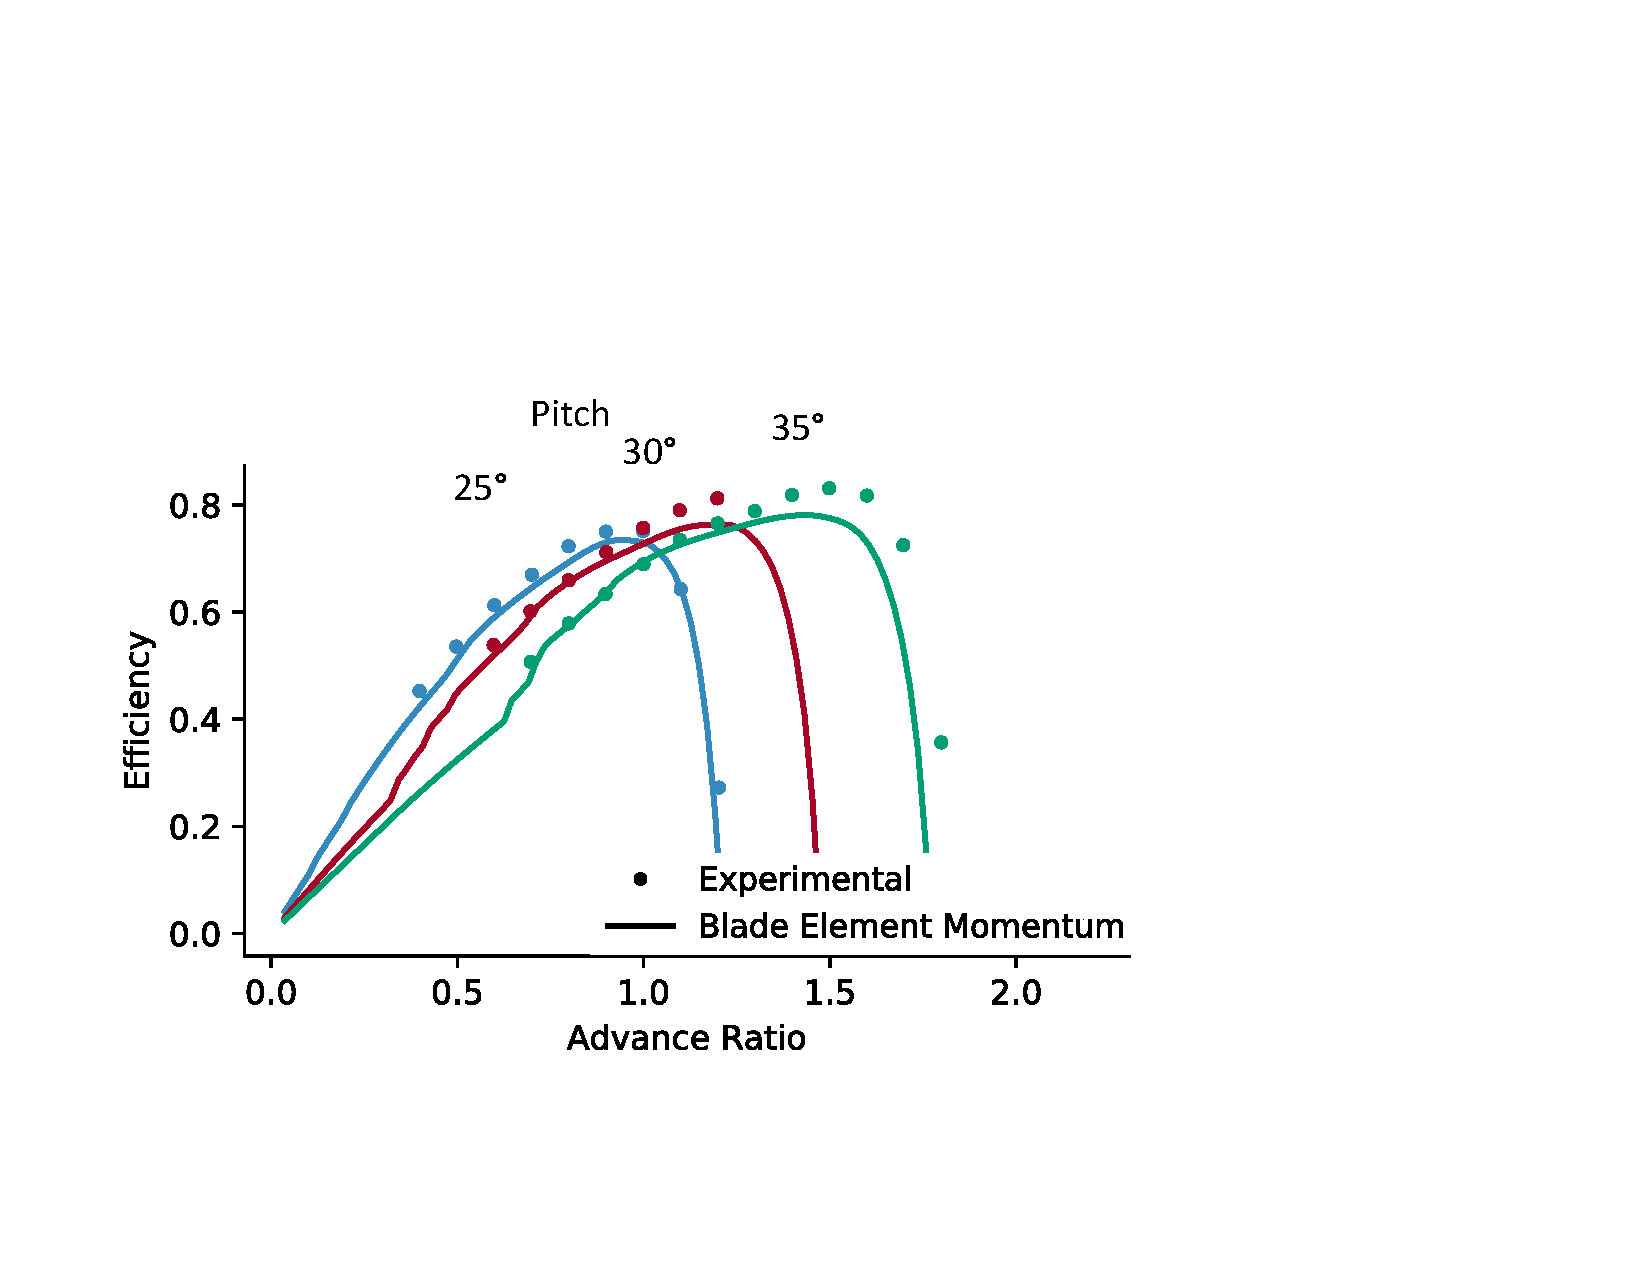
\includegraphics[trim={2.0cm 3.75cm 8.75cm 6.5cm},clip,width=3.0in]{ETA_propval}
    \caption{Comparison of propeller efficiency with data collected by Epema~\cite{epema} and our BEM model using XFOIL airfoil data. A maximum error of 5\% can be seen in the normal regions of operation.}
    \label{fig:eta_prop}
\end{figure}


\subsection{Propeller Noise}

\label{sec:prop_noise}
In our early versions of this work~\cite{Moore:2018aa} we used propeller tip speed as a surrogate for noise. We showed that the takeoff performance of a DEP STOL aircraft was much less affected using tip speed constraints than what we show in this current work using semi-experimental blade noise. While tip speed captures the magnitude change in noise for a set number of propellers, it is not enough to enable comparison of noise between aircraft designs with different numbers of propellers and the associated blade design changes. In this study we model propeller noise using code\footnote{BPM.jl on BYU FLOW Lab GitHub \href{https://github.com/byuflowlab/BPM.jl}{https://github.com/byuflowlab/BPM.jl}} developed and validated by Tingey~\cite{eric_noise}, which uses acoustic modeling techniques by Brooks, Pope, and Marcolini (referred to as the BPM equations)~\cite{BROOKS:1986aa, BPM}.

~\Cref{fig:noise_contour} shows a graphical representation of the A-weighted noise profile for an example 8 propeller case in climb at 50 ft with respect to a ground observer. Because this is a comparative conceptual study, we use this semi-empirical noise model as an approximate calculation for the major components of propeller noise. More detailed use of this model would require calibration and validation specific to the application, as well as other forms of noise generated by the rest of the aircraft such as from the wing, fuselage, electric motors, and motor controllers. However, this model captures the main portion of the total noise generation of an electric aircraft enabling us to make a better a comparison between designs with different numbers of propellers, blades, and blade geometry.

\begin{figure}[h!]
    \centering
    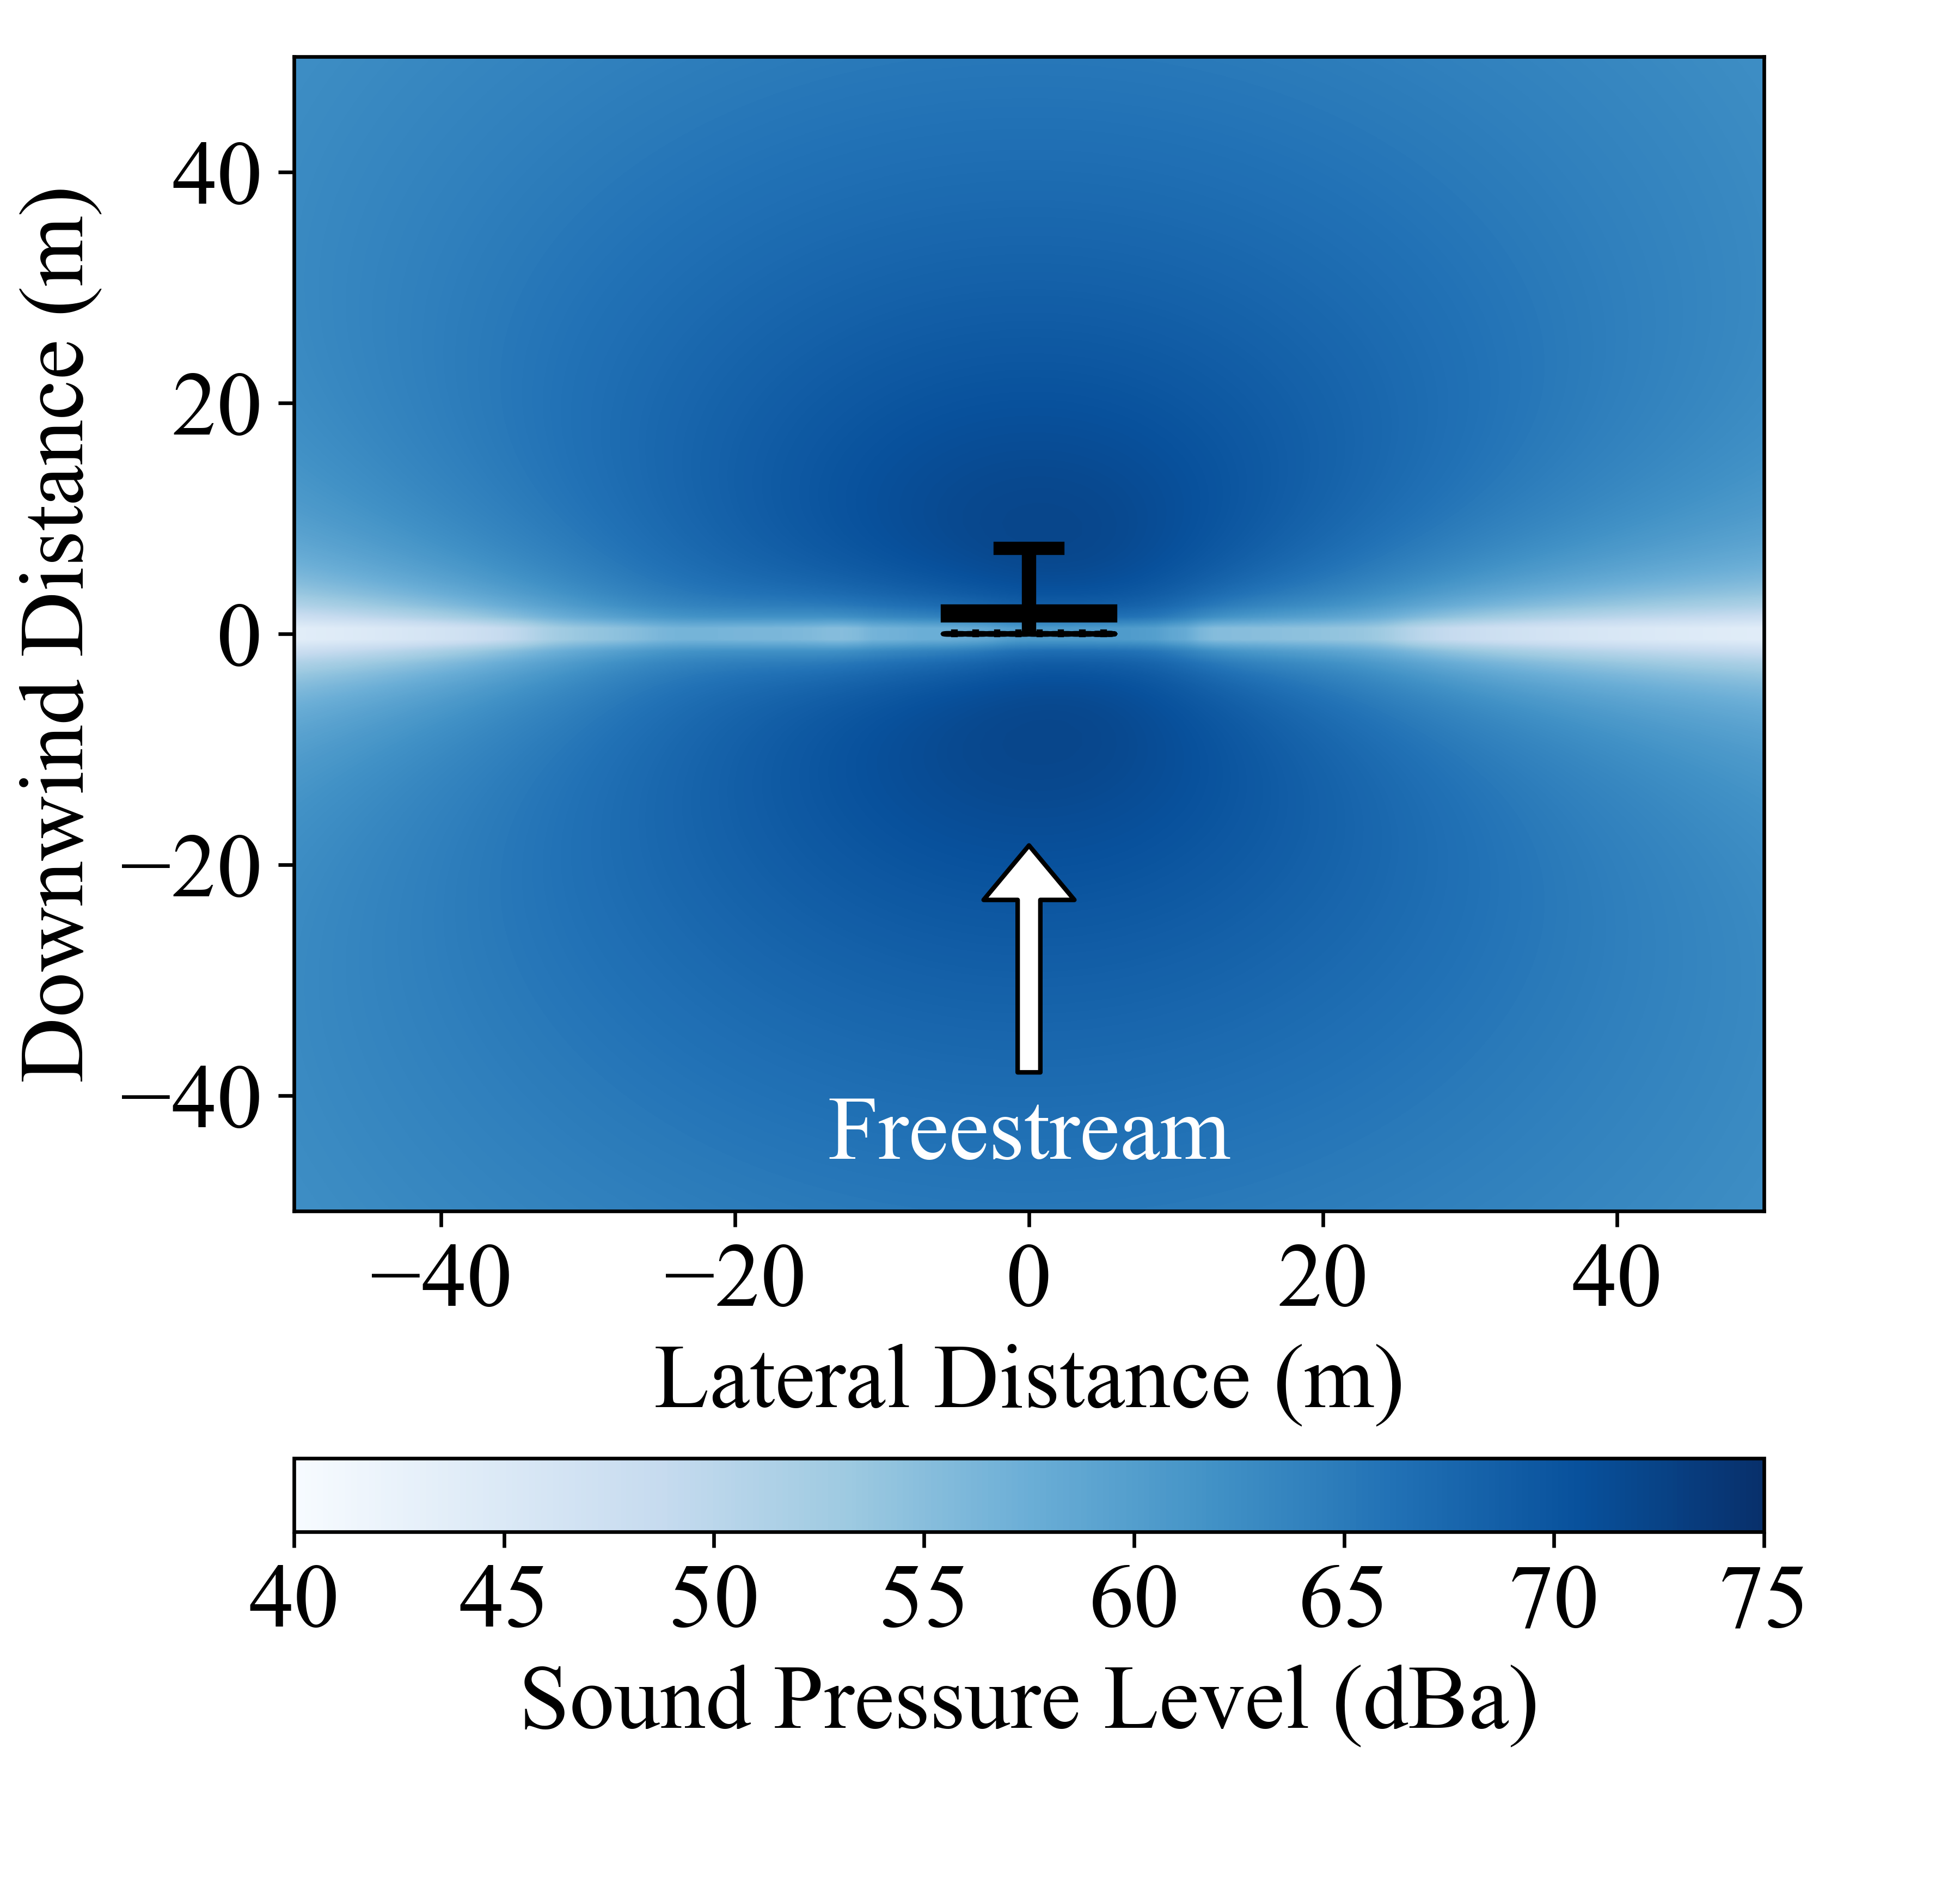
\includegraphics[trim={0cm 1cm 0cm 0cm},clip,width=3.0in]{noise_contour.png}
    \caption{Noise profile of example 8 propeller case in climb at 50 ft with respect to a ground observer. (Airframe included for reference.)}
    \label{fig:noise_contour}
\end{figure}

\subsection{Composite Structures}


Since our objective is to minimize takeoff distance, the propellers will be subject to very high loading to achieve the thrust required on takeoff. To achieve a more realistic total design, we need to include the structural constraints and their effects on the aerodynamic design. These constraints ensure that the blade design and structure meets failure criteria as well as minimum and maximum composite thicknesses. A by-product of this is that the total propeller mass can be more accurately predicted, which in some cases can be as high as 6\% of the allowable propulsion and battery mass.

\subsubsection{Propeller Blade Composite Layup}

The composite layup for the propellers is defined as a shell with two ply types: unidirectional (or uni) carbon prepreg along the blade span and bidirectional weave (or weave) oriented at 45$^{\circ}$. To enable gradient-based optimization for this conceptual study, the plies are modeled with continuous thicknesses.

We use PreComp\footnote{PreComp.jl on BYU FLOW Lab GitHub \href{https://github.com/byuflowlab/PreComp.jl}{https://github.com/byuflowlab/PreComp.jl}} to calculate the span-variant sectional properties of the shell, which include mass, stiffnesses, and inertias. From the distributed mass, we calculate each blade mass with trapezoidal integration and scale it according to the number of propellers and blades. PreComp also calculates the structural centers of shear, mass, and tension which are needed to transform the aerodynamic forces from the aerodynamic center into the structural frame of reference. The relative distances between the structural centers and the aerodynamic center are used to transform the aerodynamic forces at the aerodynamic center of each section, calculated by BEM, into the structural frame of reference.

\subsubsection{Linear Finite Element Analysis}


With the propeller blade distributed stiffnesses calculated from PreComp, we use linear beam finite element theory~\cite{pbeam},\footnote{BeamFEA.jl on BYU FLOW Lab GitHub \href{https://github.com/byuflowlab/BeamFEA.jl}{https://github.com/byuflowlab/BeamFEA.jl}} to model the blade. This is done with the beam fixed at the hub and the propeller aerodynamic loads distributed along the blade. For this study, strains are calculated at 10 evenly spaced points around the airfoils at 8 sections along the blade using a thin shell approach.

\subsubsection{Composite Frame of Reference Stress}


To calculate stresses in the composite frame and in turn first ply failure, we use a thin shell calculation with the composite centerline strain for all layers. Calculating composite stress in the composite frame of reference is a multi-step process including calculating the shear strain and laminate stress in the beam frame of reference, then transforming the stress into the ply frame of reference~\cite{Kassapoglou:2013aa}.

\subsubsection{Material Properties}

For reference, the composite material properties used are included in \cref{tab:matprop}. The materials included are the carbon fiber reinforced plastic (CRFP) unidirectional (uni) and weave used in the results of this study. The units and description of the properties used are as follows: first axis modulus of elasticity $e_1$ (Pa), second axis of elasticity $e_2$ (Pa), shear modulus $g_{12}$ (Pa), Poisson's ratio $\nu$, density $\rho$ (kg/$m^3$), first axis failure strength in tension $x_t$ (MPa), second axis failure strength in tension $y_t$ (MPa), first axis failure strength in compression $x_c$ (MPa), second axis failure strength in compression $y_c$ (MPa), shear failure strength $s$ (MPa), single ply thickness $t$ (mm).\\

\setlength{\tabcolsep}{6pt}
\begin{table}[htbp]
    \begin{center}
        \caption{Composite Material Properties}
        \label{tab:matprop}
        \begin{tabular}{lccccccccccc}%rrrrrrrrrrr} % <-- Alignments: 1st column left, 2nd middle and 3rd right, with vertical lines in between
            \textbf{Name} & \textbf{$e_1$} & \textbf{$e_2$} & \textbf{$g_{12}$} & \textbf{$\nu$} & \textbf{$\rho$} & \textbf{$x_t$} & \textbf{$y_t$} & \textbf{$x_c$} & \textbf{$y_c$} & \textbf{$s$} & \textbf{$t$} \\
            \midrule
            Uni & $1.75$e$11$ & $0.8$e$10$ & $5.0$e$9$ & 0.3 & 1600.0 & $8.060$e$8$ & $6.719$e$8$ & $2.962$e$7$ & $1.667$e$8$ & $5.357$e$7$ & $0.152$ \\
            Weave & $8.5$e$10$ & $8.5$e$10$ & $5.0$e$9$ & $0.1$ & $1600.0$ & $2.821$e$8$ & $1.186$e$8$ & $2.592$e$8$ & $1.250$e$8$ & $3.125$e$7$ & $0.218$ \\

        \end{tabular}
    \end{center}
    \vspace{-12pt}
\end{table}


\subsubsection{Material Failure}

We use the Tsai-Wu failure criteria~\cite{Tsai:1971aa} to predict first ply laminate failure. Prior to applying the Tsai-Wu failure criteria, we apply safety factors, material scatter knockdown factors, and barely visible impact damage (BVID) knockdown factors. The material scatter knockdown factors are calculated for the carbon fiber uni and weave based on A-basis values from Tomblin et al.~\cite{tomblin:2002aa,tomblin:2002ab}. They are shown in \cref{tab:scatterfactor} for reference and have already been applied to the uni and weave in \cref{tab:matprop}. The BVID knockdown factor was chosen to be 0.65~\cite{Kassapoglou:2013aa} and the safety factor to be 1.5. To predict buckling, we assume long, simply-supported plates and calculate buckling strain with respect to the composite stiffness as described by Johnson et al~\cite{JOHNSON:1994aa}. \\

\setlength{\tabcolsep}{5pt}
\begin{table}[htbp]
    \begin{center}
        \caption{Material Scatter Knockdown Factors}
        \label{tab:scatterfactor}
        \begin{tabular}{cccccc}
            \midrule
            Material & \textbf{$k_1^+$} & \textbf{$k_1^-$} & \textbf{$k_2^+$} & \textbf{$k_1^-$} & \textbf{$k_{12}$} \\
            %      $\alpha$ & $\beta$ & $\gamma$ \\
            \midrule
            T300/934 tape & 0.625 & 0.762 & 0.803 & 1.0 & 0.920 \\
            T300/934 fabric & 0.764 & 0.776 & 0.719 & 0.859 & 1.0 \\
        \end{tabular}
    \end{center}
    \vspace{-12pt}
\end{table}

\subsection{Waked Wing Modeling}

\label{sec:VLM}

The vortex lattice method (VLM) is a discretized lifting line theory that calculates the inviscid lift and lift-induced drag for non-uniform freestream and geometry~\cite{Lan:1974aa}. Typically the method is implemented with a uniform freestream that is applied independently at each vortex boundary condition. In order to account for the propeller on wing effects, we have included the propeller axial and tangential velocity distributions in the boundary condition similar to that done by Veldhuis~\cite{proponwing}. To account for the propeller induced drag on the system we include the swirl loss factor as described by Veldhuis as well.

Specifically regarding the tangential, or swirl velocity, induced by the propeller, it is important to note that not all of this velocity is applied to the boundary condition in the vortex lattice method~\cite{Alba:2017aa}. Neglecting a correction on the swirl velocity over-predicts its effect on the wing lift distribution as previously noted by Hunsaker~\cite{Hunsaker:2006aa} with the local lift coefficient being over-predicted by as much as 6x. Additionally, the optimal blown lift distribution is non-elliptical~\cite{Veldhuis2004}, which makes the propeller on wing interaction critical for design.

\subsubsection{Stall}

We use critical section stall theory by imposing a 20\% reduction in the allowable local lift coefficient on the last 5\% of the wing span. The allowable local lift coefficient, normalized by the local velocity is 2.4 for takeoff and 1.2 during cruise. The local lift coefficient stall constraint of 2.4 is a surrogate for extended flaps with a zero lift angle of attack at -14$^\circ$ for a single slotted flap at 30$^\circ$ deflection~\cite{Abbott:2012aa}. The local lift coefficient of 2.4 is also a 10\% margin below the maximum local lift coefficient of the flap configuration chosen.


\subsubsection{Prop on Wing Smoothing}

While vortex lattice methods can be evaluated rapidly, their discrete panels can create difficulties with gradient-based optimization. This problem arises for this study because we are interested in exploring different propeller sizes as a design variable. As the propeller diameter changes, the propeller wake blankets a different number of VLM panels. Specifically, as the wake moves over a new control point, the predicted forces and moments change in a discontinuous manner.


\begin{figure}[htbp]
    \centering
    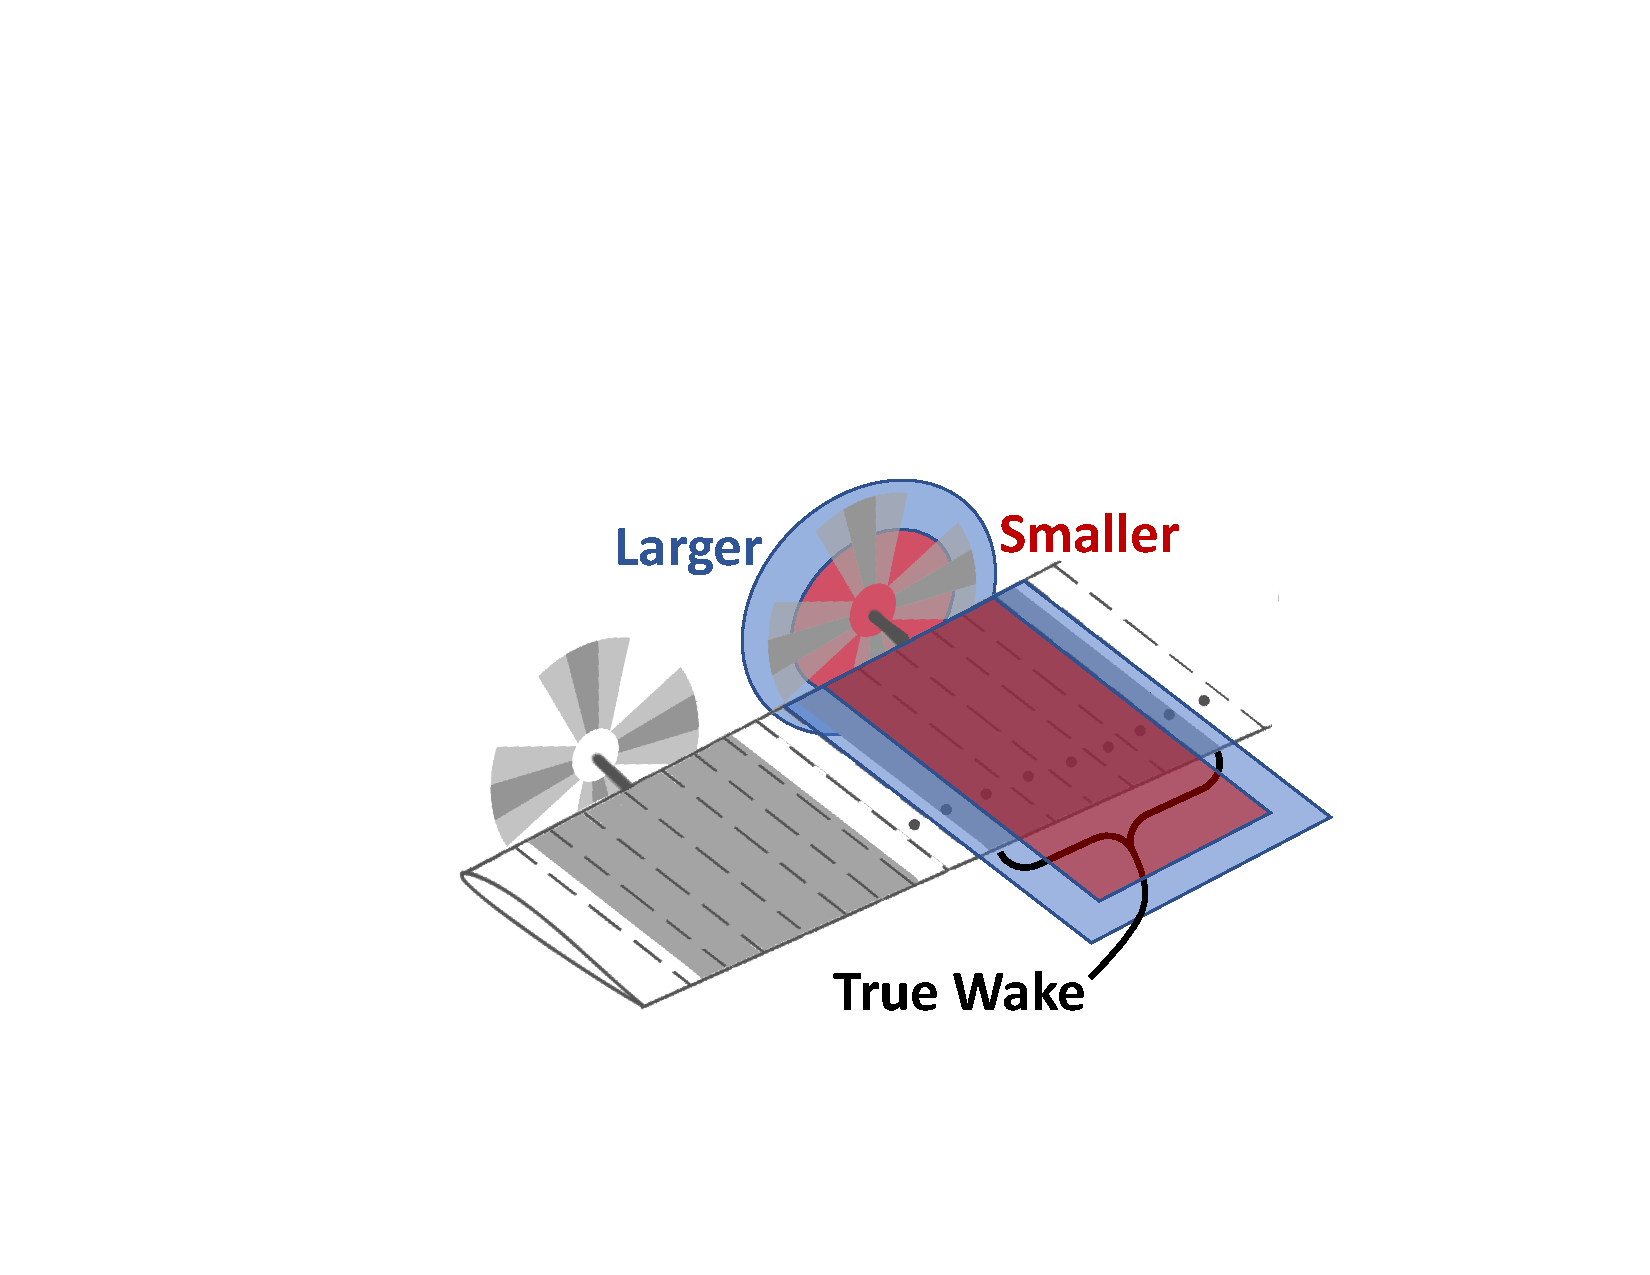
\includegraphics[trim={7.75cm 4.25cm 5.4cm 7.75cm},clip,width=3.0in]{wake-smooth4}
    \caption{Illustration of smooth evaluation of varying rotor diameter. Rotor wake is evaluated at next larger (blue) and next smaller (red) diameters waking full VLM panels. The results (including viscous drag) are linearly interpolated to the true rotor wake.}
    \label{fig:wake-smooth}
\end{figure}

To overcome the discontinuities, our methodology has two parts. First, we ensure that the center of the propeller wake is centered on a wing control point. Because the position and number of propellers are fixed during the optimization, these locations can be precomputed. Also, since the propeller and control point locations are non-dimensionalized based on the wingspan, the span could be added as a design variable for constant propeller relative locations and number of control points. Second, for each wake diameter we find the two nearest far field diameters, one smaller and one larger, that exactly cover full panels (see \cref{fig:wake-smooth}). We evaluate the VLM at both the smaller diameter and larger diameter conditions, then linearly interpolate the VLM outputs using the wake diameter (this is not the same as the rotor diameter due to wake contraction). The linear interpolation is applied to scalar values as well as arrays, such as the wing distributed lift and drag. This is particularly useful since the viscous drag can also be included in the interpolation allowing for partial waking of the VLM panels for the viscous model as well.

A comparison of the old method and new linear interpolation method can be seen in \cref{fig:smoothvlm} showing the effects on the wing lift coefficient $C_L$, and wing induced drag coefficient $C_{Di}$. The original function contains many artificial local minima, while this modified approach produces a differentiable output. While this modification does require twice the number of function calls to the VLM, it allows for rotor diameter to be directly included in the optimization. Not including the rotor diameter in the optimization increases the complexity of the problem by making the problem combinatorial or would require a variable sweep of the propeller diameter for each of the numbers of propellers tested.


\begin{figure}[htbp]
    \centering
    \subfloat[lift coefficient]{
    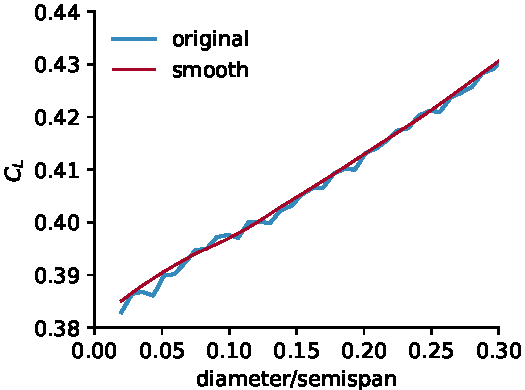
\includegraphics[width=0.45\textwidth]{smoothCL}
    \label{fig:smoothCL}
    }
    \qquad
    \subfloat[induced drag coefficient]{
    \includegraphics[width=0.45\textwidth]{smoothCDI}
    \label{fig:smoothCDI}
    }
    \caption{Comparison between the original propeller on wing VLM output and our modified approach which eliminates the artificial minima in the function space.}
    \label{fig:smoothvlm}
\end{figure}

\subsubsection{Propeller on Wing Validation}

We examined two separate validation cases for the propeller on wing interaction. The first case is from wind tunnel data of a single propeller on a straight untwisted wing by Veldhuis \cite{Veldhuis2004,proponwing} at $0^\circ$ and $4^\circ$ angle of attack. \Cref{fig:epemaval1} shows a comparison between the experimental lift coefficient and that predicted by our methodology for both angles of attack. Agreement is observed in \cref{fig:epemaval1} with a standard deviation on the error of 0.009 and 0.015 for the upper and lower curves respectively with error being greatest at the propeller slipstream boundary.

The second set of experiments comes from a separate wind tunnel experiment by Epema \cite{epema}, using a larger propeller and a tapered wing. We compare the results for the lift distribution for our VLM, the VLM developed by Epema in that same study, and the wind tunnel data. Reported error bars in the wind tunnel data are included in \cref{f:epemaval2} and are due to the dynamic nature of the propeller helical vorticies~\cite{Alvarez:2018aa}. The two VLMs tend to follow the experimental trends except where the propeller swirl velocity induces wing upwash in the half-span regions between advance ratios 0.2 and 0.3. In this region our VLM more closely matches the experimental data and overall has a standard deviation of error of 0.07 with respect to the mean experimental values.

\begin{figure}[htbp]
    \centering
    \subfloat[Lift coefficient distribution from our BEM/VLM compared to Veldhuis experimental wind tunnel data at 4 degrees (upper) and 0 degrees (lower) angles of attack.]{
    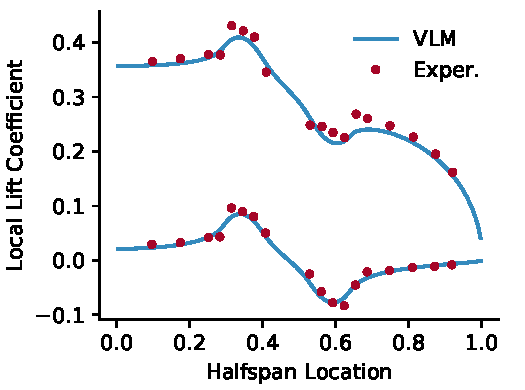
\includegraphics[width=3.0in]{Veldhius}
    \label{fig:epemaval1}
    }
    \qquad
    \subfloat[Lift distribution from our BEM/VLM compared to Epema BEM/VLM and experimental data at 4 degrees angle of attack. Error bars show one standard deviation.]{
    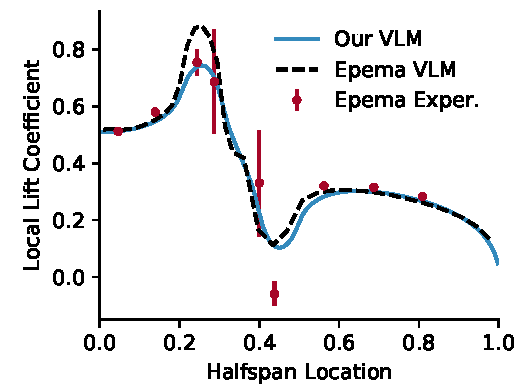
\includegraphics[width=3.0in]{Epema}
    \label{f:epemaval2}
    }
    \caption{Two validation cases for propeller on wing interaction using two different geometries.}
    \label{f:epemaval}
\end{figure}

\subsection{Electric Components Modeling}

Based on the results of this study, the motor and motor controller can fill as much as 88\% of the total available battery and propulsion mass. Additionally, a less efficient motor may require more current, and in turn a larger mass, to output the same amount of power as a more efficient motor. Therefore, with this type of aircraft problem where the mass has a significant coupled effect due to lift induced drag, mass modeling is a critical part of this conceptual design.

\subsubsection{Electric Motor}

\label{Motor}

For calculating motor efficiency and power, we use a fundamental first order motor model \cite{DrelaMotor}. Comparing the first order model to the Maxon 305013 Brushless Motor\footnote{Maxon Motors Online Catalog \href{https://www.maxonmotorusa.com/maxon/view/catalog/}{http://www.maxonmotorusa.com}, accessed 4/11/19} data, we found the efficiency, current, and required voltage to all be within 1.5\% for the nominal RPM and torque.


In order to model the motor mass, we created a linear fit to the motor data from the Astroflight\footnote{Astroflight Motors \href{http://www.astroflight.com}{http://www.astroflight.com}, accessed 4/11/19} line of motors. Astroflight motors were chosen due to the availability of data and the favorable range of both power and Kv. We found a linear relationship between the mass and the motor peak current divided by the motor $K_v$ parameter (\cref{fig:motorMass}). The line fit in \cref{eq:motorMass} shows the trend of the motor mass and with an $R^2$ value of 0.94. The motors included in this empirically-based model ranged from 1.5 kW to 15 kW and $K_v$ from 32 to 1355.

\begin{figure}[htbp]
    \centering
    \subfloat[Astroflight motor mass fit in blue with data in red. The equation for the linear fit is shown in \cref{eq:motorMass}.]{
    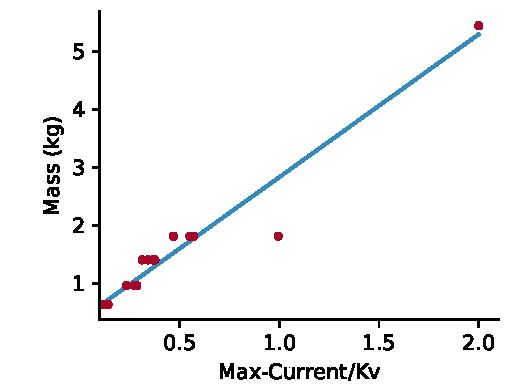
\includegraphics[width=0.45\textwidth]{motorMass3}
    \label{fig:motorMass}
    }
    \qquad
    \subfloat[Astroflight motor $I_0$ and $R_0$ fit in blue with data in red. Fit equation shown in \cref{e:motor_V0}.]{
    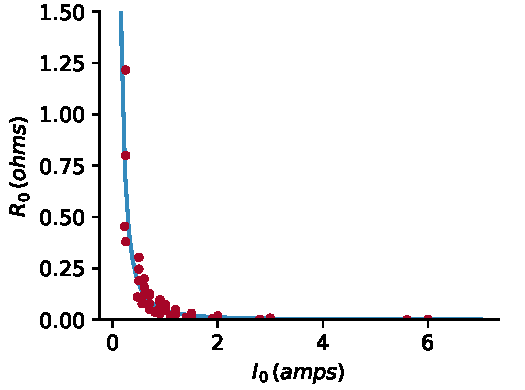
\includegraphics[width=0.45\textwidth]{I0_R03}
    \label{f:MparamFits}
    }
    \caption{Data fits based on Astroflight motor data.}
    \label{fig:motorempirical}
\end{figure}



\begin{equation}
\label{eq:motorMass}
m_{motor} = 2.464\, \frac{I_{m}}{K_v}+0.368
\end{equation} \

To accurately model motor performance in addition to mass, we investigated the relationship between all of the motor parameters. We found that there were no interdependencies other than the relationship already discussed between the mass, motor peak current, and $K_v$, then the relationship between the no-load resistance and no-load current. The trend for the latter can be seen in \cref{f:MparamFits} and the accompanying fit in \cref{e:motor_V0} with an $R^2$ value of 0.93.

\begin{equation}
\label{e:motor_V0}
R_0 = 0.0467(I_0)^{-1.892}
\end{equation} 


\subsubsection{Linearized Battery and Motor Controller Masses}

Due to the scope and nature of this comparative conceptual design study, we used a simplified approach to model the motor controller and battery masses. The motor controller model for mass was assumed to be linear based on the specific power of 22,059 W/kg taken from the Astroflight high voltage motor controller. Efficiency of the motor controller was assumed to be a constant 97\%. The battery was modeled with a specific energy parameter of 300 Wh/kg, representative of a mid-life, currently available Li-S battery~\cite{Mikhaylik:2010aa}.


\section{Aircraft Takeoff Performance}
\label{sec:Performance}

While it would be more ideal to model the full balanced field length, as will be discussed in the results section, the time to liftoff is on the order of seconds. This means that the pilot reaction time of approximately one second\footnote{\label{reaction_time}FAA Takeoff Safety Training Aid \href{https://www.faa.gov/other\_visit/aviation\_industry/airline\_operators/training/media/takeoff\_safety.pdf}{https://www.faa.gov/other\_visit/aviation\_industry/airline\_operators/training/media/takeoff\_safety.pdf}, accessed 4/11/19} could make an aborted takeoff infeasible before liftoff. A revised balanced field length calculation for this type of aircraft including concepts discussed by Patterson~\cite{Patterson:2017aa} may be in order. Due to this uncertainty in the full field length calculation for this type of aircraft, we focused on the minimum conceptual takeoff distance including ground roll, transition, and climb. For simplicity and as a conservative factor we did not include the beneficial effects of ground effect in our takeoff distance calculations.

In our final results for this type of STOL aircraft, we found ground roll distance alone accounts for about 20\% of the total distance to clear a 50 ft obstacle. Additionally, the transition distance from liftoff to steady climb must be accounted for due to the large flight path angles encountered and can exceed 30\% of the total takeoff distance. A graphical representation of the three parts of takeoff can be seen in~\cref{f:takeoff}, where the figure is scaled to represent an example 8 propeller case typical of the results. In light of these requirements, we review the dynamics of aircraft acceleration for constant power, then for transition, and finally for steady climb, all adapted for high angles of attack. We also review the aircraft range calculation.


\begin{figure}[htbp]
    \centering
    \includegraphics[width=3.5in]{takeoff}
    \caption{Example takeoff profile scaled to represent a sample 8 propeller case. Takeoff transition becomes significant when the flight path angle is greater than a few degrees.}
    \label{f:takeoff}
\end{figure}

\subsection{Ground Roll Distance}

\label{GroundRollDistance}

To model the ground roll, or acceleration distance, we use an approach similar to Anderson's constant thrust approach~\cite{Anderson:2015aa}. His approach assumes the aircraft starts from rest and is accelerated to the takeoff speed with a constant thrust and mass, and an averaged drag. While turbine engine based propulsion is assumed to have a constant thrust during takeoff, electric propulsion is assumed to have a constant power during takeoff. Because of this, a slight variation in Anderson's takeoff rolling distance equation is required. Beginning with the same assumptions (constant mass, acceleration from rest, and average drag) as in his takeoff performance equation, we modify the derivation to assume a constant power during takeoff resulting in the following integration for takeoff roll distance with the ground roll distance $s_{GR}$, the total mass $m$, the freestream velocity at liftoff $V_{\infty}$, and the net power output $P_{net,out}$ (total power less power due to drag at liftoff for conservatism). (See \cref{e:GR})

\begin{equation}
    \label{e:GR}
    s_{GR} = \frac{m V_{\infty}^3}{3P_{net,out}}
\end{equation}

\subsection{Steady Climb}

We model aircraft climb with the simple steady climb equation for the flight path angle~\cite{Anderson:aa}. However, we correct the thrust for angle of attack since the large amounts of thrust become significant at high angles of attack. The simple correction in \cref{e:flightpathangle} includes the flight path angle $\gamma$, thrust $T$, total drag $D$, mass $m$, angle of attack $\alpha$, and gravity $g$.

\begin{equation}
    \label{e:flightpathangle}
    \gamma = \sin^{-1}\Bigg(\frac{T cos{\alpha} - D}{m g}\Bigg)
\end{equation}


\subsection{Transition}


To fully characterize the transition path, we could use the x and y components of force and Newton's second law and numerically integrate the acceleration to find the exact path over time. However, this approach becomes infeasible for design optimization. Numerical integration would require thousands of additional evaluations, which would make an optimization that normally takes around 20,000 function evaluations or just a few hours, take several thousand times that, or months to solve. A simpler approach to full dynamic simulation is to approximate the transition via a circular path and assume that the flight speed, lift, drag, angle of attack, and thrust are constant~\cite{Mair:aa}. Using the dynamic equation for a circular path due to acceleration from excess lift allows us to calculate a radius and in turn the traversed distance.

\subsection{Range}


To model range, we used a non-standard formulation in the propulsion frame of reference as opposed to the airframe frame of reference. This was done to increase the convergence rate of the optimization. This slight variation of the more typically used range equation~\cite{Anderson:2015aa} is shown in \cref{eq:range1} with range $R$, battery mass $m_b$, battery specific energy $e$, thrust $T$, and propulsion efficiency $\eta_{p}$.

\begin{equation}
    \label{eq:range1}
    R = \frac{m_{b} \, e \, 3600 \, \eta_{p}}{T}
\end{equation}


%%%%%%%%%%%%%%%%%%%%
%%  END METHODOLOGY
%%  START ANALYSIS SETUP
%%%%%%%%%%%%%%%%%%%%


\section{Optimization Setup}
\label{chp:OptimizationSetup}


In this study, we explore tradeoffs between takeoff distance and cruise speed for the general parameters of the baseline Tecnam p2006t aircraft\footnote{\label{p2006t} P2006T Aircraft Flight Manual \href{http://www.tecnamair.com/wp-content/uploads/2017/04/P2006T-12-w-NUEVO.pdf}{http://www.tecnamair.com/wp-content/uploads/2017/04/P2006T-12-w-NUEVO.pdf}, accessed 4/11/19}, but with continuously powered distributed propellers in a retrofit configuration. We chose to keep the airframe, wing, and max takeoff weight unchanged to keep this conceptual study a retrofit of the existing aircraft. Also, to increase efficiency during takeoff and cruise, we include variable pitch propellers, but limit the allowable tip Mach number to 0.8 to stay reasonably within the XFOIL's compressibility correction equation limits.

Using our optimization framework, we investigate only the effects of the propulsion system, while assuming no changes in trim drag due to an unchanging maximum takeoff weight (MTOW) and assumed use of battery mass for ballast if needed. We vary the number of propellers ranging from 2 until the performance degrades at 32 propellers. We set up the VLM model with 120 control points per half-span. We design the propellers by changing the blade chord, twist, radius, and number of blades while maintaining the same airfoil profile (the Eppler 212 low Reynolds number airfoil). Propellers were modeled as rotating inboard-up due to lower propeller on wing induced drag losses as opposed to outboard-up~\cite{Kroo:1986aa}. In order to model ground roll, transition and climb, and cruise performance, we use three sets of the four variables including RPM, pitch, angle of attack, and battery capacity. We use only one set of variables for the propeller geometry and motor parameters, and size the electronics based on the highest-power case (using a smooth-max function to avoid discontinuities). Battery capacity is modeled as a design variable to avoid an inner convergence loop since the total aircraft mass is required to calculate the battery energy and in turn, battery mass needed. Energy constraints on the three stages (ground roll, transition and climb, and cruise) allow the battery mass to converge at the proper total value.

\subsection{Framework}

\label{sec:Framework}


\Cref{f:frameworkplan} shows the general modeling framework used to evaluate the aircraft performance. In the figure, colors distinguish the design variables (red), models (green) and constraints (blue). The constraints include factors on flight and structural requirements as well as modeling limitations. These include a constraint on the propeller blade local angle of attack to help with convergence, lift greater than weight, and thrust greater than drag at each respective stage but with thrust allowed to be in excess where needed for takeoff performance. Other constraints include battery sizing, maximum propeller tip speed mach number, maximum sound pressure level (SPL), local lift distribution for stall, propeller tip separation to prevent overlapping, MTOW, range, cruise speed, composite failure, and buckling stress.

\begin{figure}[h!]
    \centering
    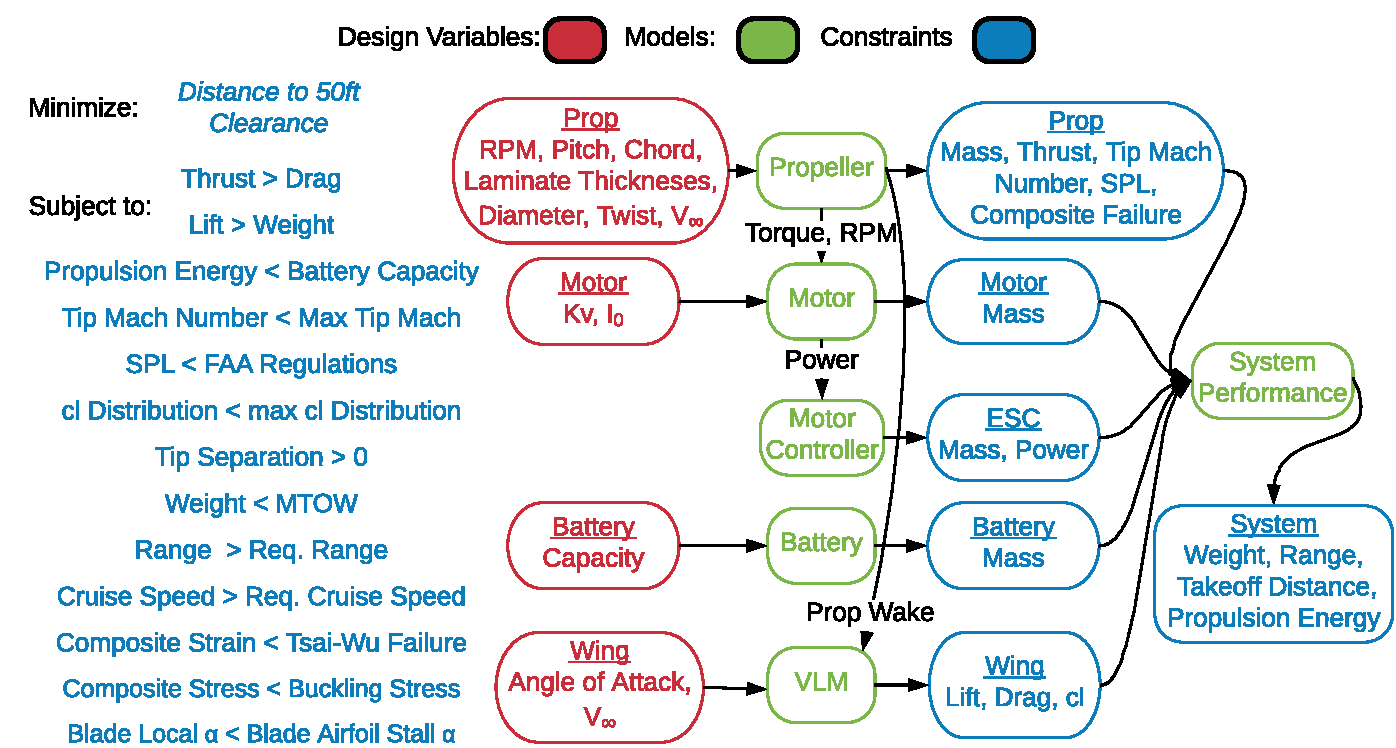
\includegraphics[trim={0.35cm 0cm 0.0cm 0cm},clip,width=0.99\textwidth]{OptDiagram-3}
    \caption{Optimization framework with design variables in red, models in green, and outputs in blue. To account for acceleration, transition and climb, and cruise phases, we ran the analysis framework three times with repeated variables for angle of attack ($\alpha$), pitch, RPM, and velocity. }
    \label{f:frameworkplan}
\end{figure}

\setlength{\tabcolsep}{5pt}

The design variables used and touched on in \cref{f:frameworkplan} total to 35. We chose the upper and lower bounds for each design variable to help the optimization convergence by limiting the available design space to not include extreme design values. As an example, the lower bound on the wing angles of attack were set to be much lower than the typically converged value, but do not allow for values at which the constraints would always be violated. During development of the final solutions, the upper and lower bounds were updated to reflect this technique, especially when a design variable was at a bound constraint.


Using the Julia programming language, the full propeller and wing, propeller aerostructural, and propulsion system codes run in an average of approximately 0.26 seconds without the noise model and 0.5-3.5 seconds with the noise model depending on the total number of blades. This means optimizations usually converge in the order of hours. The gradient based optimization algorithm used was the Sparse Nonlinear OPTimizer (SNOPT)~\cite{snopt}.

\subsection{Baseline Aircraft}

\label{Short Haul Commuter}

As mentioned previously, we chose the Tecnam p2006t aircraft because of the work already being done to exchange the two engines for electric motors~\cite{Borer:2016aa}. Our intent is to show the conceptual feasibility of electrifying an existing aircraft as a possible near term solution to the urban ODM problem, thus potentially simplifying certification and safety requirements. \Cref{tab:short_haul} shows the main design parameters and limitations of the aircraft.

\setlength{\tabcolsep}{10pt}

\begin{table}[htbp]
    \begin{center}
        \caption{Baseline Tecnam p2006t aircraft{\footref{p2006t}}}
        \label{tab:short_haul}
        \begin{tabular}{lrr} % <-- Alignments: 1st column left, 2nd middle and 3rd right, with vertical lines in between
            \textbf{Parameters} & \textbf{Tecnam p2006t} & \textbf{Present Study} \\
            \midrule
            Propulsion Designed For: & Cruise & Short Takeoff   \\
            \midrule
            MTOW & 1230 kg  & 1230 kg   \\
            Wet Useful Load & 257 kg & 245 kg   \\
            Engines \& Fuel & 289 kg & 0 kg   \\
            Propulsion \& Battery Allowance & 0 kg & 301 kg   \\
            Cruise Speed & 77.3 m/s & 22, 45, 67 m/s  \\
            Range & 1239 km & 50 km  \\
            Max Power & 140 kW & 100-600 kW \\
            Flight Path Angle & 3.5 deg & 7-40 deg  \\
            Noise & 67 dB(a) & 60-76 dB(a)  \\
            Wing Area & 13.47 m$^2$  & 13.47 m$^2$   \\
            Wingspan & 11.67 m & 11.67 m  \\
            Aspect Ratio & 10.1 & 10.1  \\

        \end{tabular}
    \end{center}

\end{table}

Because of the relatively low energy density of the electric system, we reduced the conceptual wet useful load to the level of the Cessna 172 in addition to using all of the mass from the engines and fuel for the batteries and electric propulsion system. We chose a 50 km range requirement as the minimum range this type of urban transport aircraft would need to begin to be useful. This was based on the approximate radius of major urban areas such as Dallas, Texas, and New York City, and also to address the very limited mass available for the propulsion system and battery. Altitude at takeoff for the atmospheric properties was set at sea level, and cruise was set at the minimum allowable altitude of 500 ft (155 m).



%%%%%%%%%%%%%%%%%%%%
%%  END ANALYSIS SETUP
%%  START RESULTS
%%%%%%%%%%%%%%%%%%%%

\section{Results}
\label{chp:Results}


For our results, we look at two parameter sweeps, or Pareto fronts, regarding the critical tradeoffs between takeoff distance, cruise speed, and noise. First we investigate the effect of cruise speed with a constant range and maximum noise level. Second, we investigate the effect of maximum noise level with a constant cruise speed and range. As previously discussed in~\cref{sec:Performance}, we present the conceptual minimum takeoff distance as opposed to a balanced field length.

\subsection{Cruise Speed Sweep}

\label{CruiseSpeedSweep}

The cruise speed constraints we explore are between the minimum speed and recommended cruise speed for the Tecnam p2006t. These nonlinear constraints are formulated to be greater than 50, 100, and 150 mph (22, 45, and 67 m/s) at noise levels less than the Federal Aviation Administration (FAA) regulation of 76 dBa (discussed in \cref{sec:noise}). \Cref{fig:takeoff_speed} shows the minimum takeoff distance Pareto fronts for varying numbers of propellers and cruise speed constraints. Based on the results of the figure, DEP clearly benefits the takeoff distance with the best high cruise speed case, the 16 propeller case, reducing the takeoff distance to less than half that of the 2 propeller case. Across all cases, excellent theoretical minimum takeoff performance is observed while meeting all other constraints. Predicted noise levels for all cases are below the 76 dBa level. Also, for the 22 m/s case, the cruise speed constraint is not active (indicated by the greater-than symbol) meaning that the converged solutions satisfy the constraint by achieving a higher cruise speed than the minimum bound constraint. The 2, 4, 8, 16, and 32 propeller cases converge to 34.6, 31.3, 33.1, 31.4, and 25.7 m/s respectively.

\begin{figure}[htbp]
    \centering
    \includegraphics[trim={0.3cm 0cm 0.0cm 0cm},clip,width=3.0in]{takeoff_speed}
    \caption{Cruise speed and number of propellers effect on minimum takeoff distance to clear a 50 ft obstacle. DEP designs satisfy the same takeoff constraints in less than half the distance.  Greater-than symbol indicates cruise speed constraint was not active. }
    \label{fig:takeoff_speed}
\end{figure}

At these takeoff distances, there are thousands of potential STOL airfield locations within major city limits~\cite{Courtin:2018aa}, meaning that DEP applied to STOL urban transport could be a feasibility even in the immediate future. If we next focus on only the ground roll distance part of the takeoff, as shown in \cref{fig:accel_speed}, we can start to make some inferences regarding the takeoff requirements with no obstacle clearance, such as the top of a building. Keeping in mind the limitations of the ground roll distance calculation as described in \cref{GroundRollDistance}, the number of potential urban locations for full balanced field length takeoff strips raises to the tens of thousands~\cite{Courtin:2018aa}. As will be discussed in the future work section, this study is intended to be a mid-fidelity conceptual feasibility study, indicating further studies in the area are needed to access things such as blown wing stall, landing approach, and powered deceleration.

\begin{figure}[htbp]
    \centering
    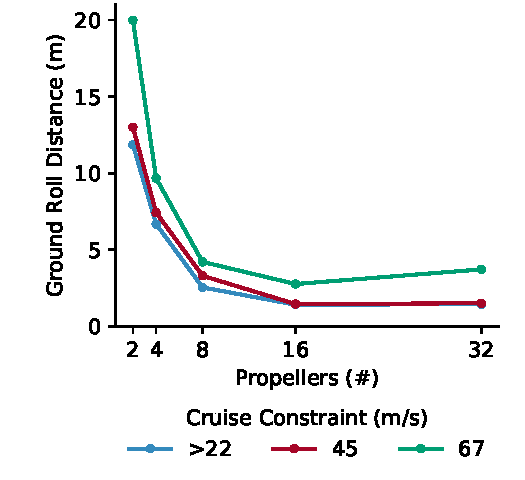
\includegraphics[trim={0.3cm 0cm 0.0cm 0cm},clip,width=3.0in]{Accel_Speed}
    \caption{Cruise speed and number of propellers effect on resulting ground roll distance to liftoff. }
    \label{fig:accel_speed}
\end{figure}


At the fundamental level of short takeoff, the two main factors in play are increased thrust and increased lift coefficient. These factors are also at the root of the increase in takeoff distance between the 16 and 32 propeller cases seen in \cref{fig:takeoff_speed,fig:accel_speed}.


\subsubsection{Augmented Thrust}


The main factor contributing to such a short takeoff distance for all cases shown in \cref{fig:takeoff_speed} is total thrust. The net thrust generated is in some cases as high as 80\% of the aircraft weight (\cref{fig:Climb_Thrust2Weight}). This is due to the relatively large propeller area as well as the inclusion of variable pitch high solidity propellers, which enables much higher thrust at low speeds. This high thrust is also possible, from a battery capacity perspective, due to the short time required for takeoff. The large power required to generate such a large amount of thrust does not significantly contribute to the battery mass. For all cases, the energy for takeoff as described in~\cref{chp:OptimizationSetup} is less than 1.5\% of the total flight energy. The optimizer takes advantage of the highly power-dense electrical components for a short period of time to significantly improve the takeoff objective. This results in an optimum at the system level, including the tradeoffs between battery mass, propulsion mass, and propulsion efficiency including the propellers' effect on the wing efficiency.



\begin{figure}[H]
    \centering
    \subfloat[Climb net thrust to weight. Total climb net thrust in excess of 80\% of the aircraft weight when the constraints on cruise speed are inactive.]{
    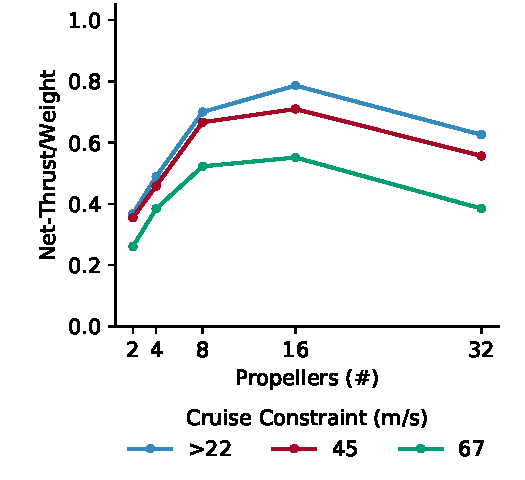
\includegraphics[trim={0.3cm 0cm 0.0cm 0cm},clip,width=3.0in]{Climb_NetThrust2Weight}
    \label{fig:Climb_Thrust2Weight}
    }
    \qquad
    \subfloat[Battery mass fraction of total aircraft mass. Increases with increasing number of propellers to satisfy range constraint at a decreased propulsion efficiency.]{
    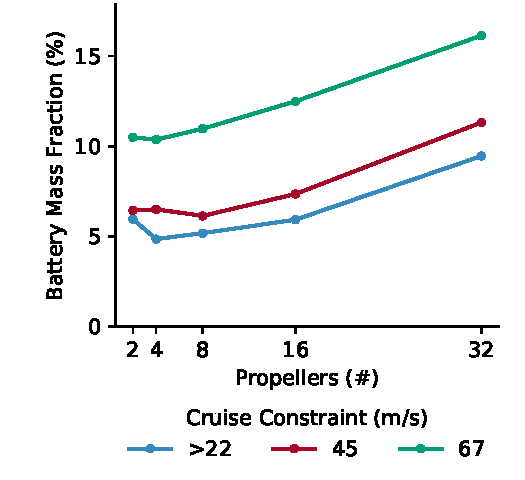
\includegraphics[trim={0.3cm 0cm 0.0cm 0cm},clip,width=3.0in]{Battery_Mass_Fraction}
    \label{fig:Battery_Mass_Fraction}
    }
    \caption{Tradeoff between battery mass and propulsion mass, or ability to generate thrust.}
    \label{fig:Thrust_Battery}
\end{figure}



After 16 propellers, the takeoff distance increases due to decreased propulsion efficiency in combination with active cruise speed, range, and MTOW constraints. With increasing number of propeller blades, the propeller efficiency drops due to the modeled tip losses with the 32 propeller, 100 m/s cruise speed case dropping by as much as 10\% compared to the 2 propeller case. This decrease in efficiency directly translates to more battery required for cruise, effectively cutting into the available propulsion system mass. With the motors taking as much as 85\% of the allowable battery and propulsion mass, a 10\% increase in battery mass has the compounding effect of decreasing the possible motor power output by as much as 30\%. The tradeoff of battery mass can be seen in \cref{fig:Battery_Mass_Fraction}.



\subsubsection{Augmented Lift}


\Cref{fig:CL_climb} shows that very large lift coefficients can be achieved with a blown wing system including flaps. Such a high lift coefficient decreases the stall speed, the required takeoff rolling distance, and for a propeller system with relatively constant power, enables greater thrust at the lower speed. This decrease in stall speed is accomplished in part by the propellers increasing the dynamic pressure on the wings as well as thrust vectoring. Thrust vectoring is inherent for a propeller in line with the wing as the angle of attack is increased, but at the cost of decreased forward thrust. The

\begin{figure}[h!]
    \centering
    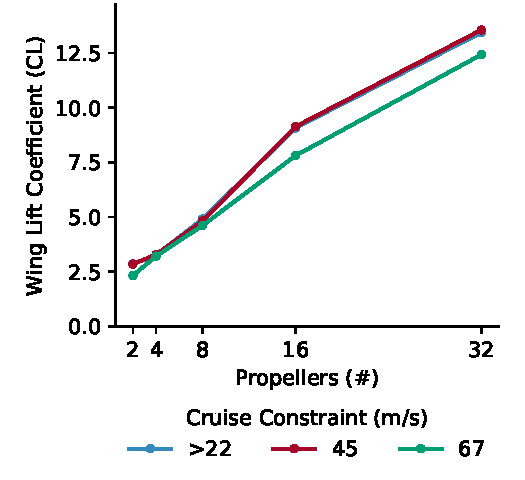
\includegraphics[trim={0.3cm 0.25cm 0.0cm 0.25cm},clip,width=3.0in]{CL_climb}
    \caption{Wing lift coefficient in the climb state with an assumed maximum local lift coefficient of 2.4 as a surrogate for extended flaps with a zero lift angle of attack at -14$^\circ$ for a single slotted flap with 30$^\circ$ deflection~\cite{Abbott:2012aa}.}
    \label{fig:CL_climb}
\end{figure}



\noindent local lift coefficient, normalized by the local velocity, remains below the specified stall constraint of a 2.4 local lift coefficient. The local lift coefficient stall constraint of 2.4 is a surrogate for extended full-span flaps with a zero lift angle of attack of -14$^\circ$ for a single slotted flap in 30$^\circ$ deflection~\cite{Abbott:2012aa}. The local lift coefficient of 2.4 is also a 10\% margin below the maximum local lift coefficient of the flap configuration chosen.

Stall is approximated with critical section stall theory by constraining the local lift coefficient. Under this modeling approach, areas within the propeller slipstream are experiencing a much lower local lift coefficient and the wing is able to achieve a much higher total freestream lift coefficient by increasing the wing angle of attack without exceeding the local lift coefficient constraint. For flight phases where a high lift coefficient is beneficial, the wing angle of attack will be increased to the point that the areas outside of the local velocity meet the local lift coefficient constraint. The extra lift from the propeller on wing interaction does cause increased induced drag, satisfying the momentum balance.

\subsubsection{Acceleration Time}


With regard to the minimum runway length, typically the balanced field length will be used where the accelerate stop distance equates the accelerate takeoff distance. For more traditional aircraft, the reaction time of about 1 second\footref{reaction_time} is a small portion of the total time. The opposite is true for this conceptual retrofit where the ground roll time is on the same order of magnitude as the reaction time, seen in \cref{fig:time_accel}. In the event of an aborted takeoff, a pilot would be well



\begin{figure}[H]
    \centering
    \subfloat[Time during acceleration portion of takeoff.]{
    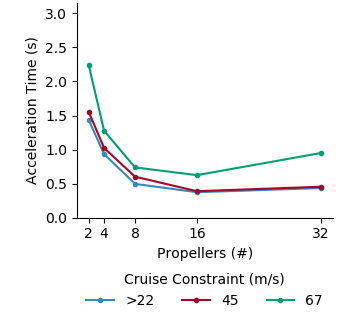
\includegraphics[trim={0.3cm 0cm 0.0cm 0cm},clip,width=3.0in]{time_accel}
    \label{fig:time_accel}
    }
    \qquad
    \subfloat[Time during transition and climb to 50 ft portion of takeoff.]{
    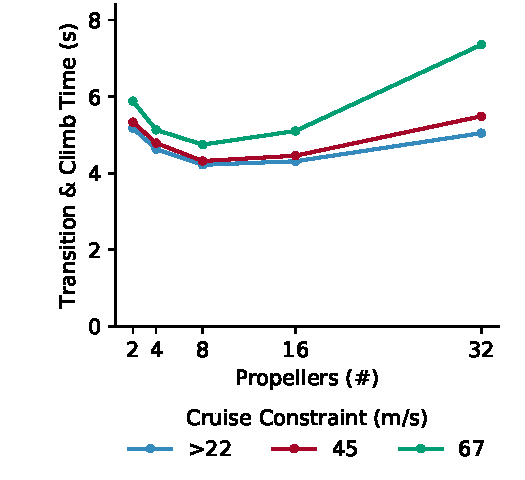
\includegraphics[trim={0.4cm 0cm 0.0cm 0cm},clip,width=3.0in]{time_tclimb}
    \label{fig:time_tclimb}
    }
    \caption{Time for takeoff maneuvers is on the same order of magnitude as a 1 second pilot reaction time\footref{reaction_time}.}
    \label{f:time}
\end{figure}

\noindent  into the transition and climb phase before reaction would be possible (see \cref{fig:time_tclimb}). To address this safety concern, the runway length could include adequate distance to transition to descent, touchdown, and deceleration.  However, this would likely require runway distances too long for inter-city services. One alternative approach, somewhat analogous to multi-engine ``Category A'' helicopter flight~\cite{LUNAAS199115}, could be taken. The aircraft could still operate from shorter runways provided adequate power and endurance were maintained to safely land at a nearby longer runway in the improbable event of critical propulsion failure. For the 16 propeller case, 14 of the electric propulsion units could fail and the system still match the power of one engine inoperable on the original p2006t.


\subsubsection{Example Propeller Design}


To give some insight into the resulting propeller design, we show one propeller from the 8 propeller, 45 m/s cruise case in \cref{f:prop8_weave_buckling}. Here we show the two active constraints for the climb phase of flight: composite weave failure shown on the upper blade and buckling failure shown on the lower blade. For all of the composite failure modes, a safety factor of 1.5 was included. From this plot, we can make several inferences regarding the propeller design. First, considering the objective of the optimization and physics of flight, the problem has an incentive to reduce the mass in all areas until propeller structural failure constraints become active. Reducing the propeller mass allows greater motor mass and in turn greater power output potential with the MTOW constraint active. Second, the weave failure constraint is active on the tension side of the blade along the leading edge. With the safety factor constraints active for the corrected material properties during the takeoff portion of the flight, the material property knockdown and safety factors may need to be reconsidered to insure an adequate true safety factor during flight in an urban setting. Third, the optimization tended toward two blades, which after re-optimizing with the integer two blades, still maintained a relatively low solidity design for the outer 50\% of the blade. We attribute this to the desirable high propeller efficiency of the case during cruise (82\%), which is quite high considering the large net thrust-to-weight produced during takeoff.

\vspace{22pt}

\begin{figure}[H]
    \centering
    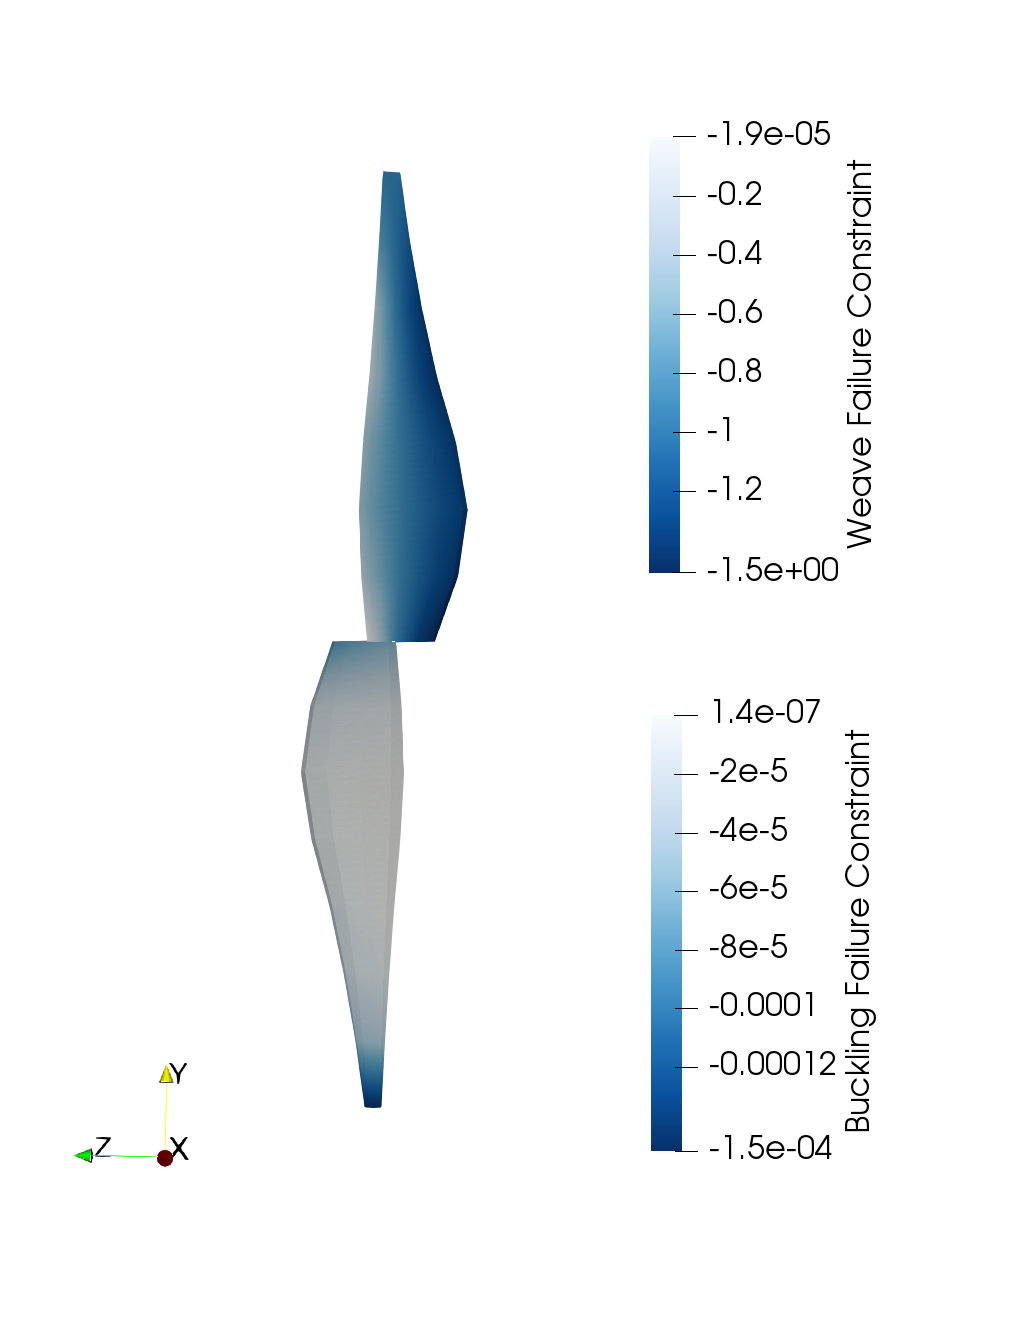
\includegraphics[trim={10.0cm 5.0cm 5.0cm 4cm},clip,angle = 0,width=2.4in]{prop8_weave_buckling}
    \vspace{0pt}
    \caption{Single propeller from the eight propeller, 45 m/s cruise case. Scaled composite weave failure constraint (upper blade) and scaled buckling failure constraint (lower blade) are active when zero or positive.}
    \label{f:prop8_weave_buckling}
\end{figure}


\Cref{f:propsize} shows the relative sizes of the optimal propeller diameter with respect to the wing span for the 45 m/s, 76 dBa noise case. Between the two and four propeller cases the propeller tip speed is the limiting factor, restricting the propeller diameter. For four propellers, the diameter is nearly as large as the two propeller case, but with four propellers the possible power output is much greater. Between the four and eight propeller cases, the total mass constraint becomes more dominant in the design space tradeoffs. This limits the power output and in turn the propeller diameter. For cases with more than eight propellers, the propeller separation constraint becomes active constraining the propellers to be effectively tip to tip. Future work may include modeling overlapping propellers and the resulting performance impacts to allow for staggered, overlapping propellers.

\begin{figure}[H]
    \centering
    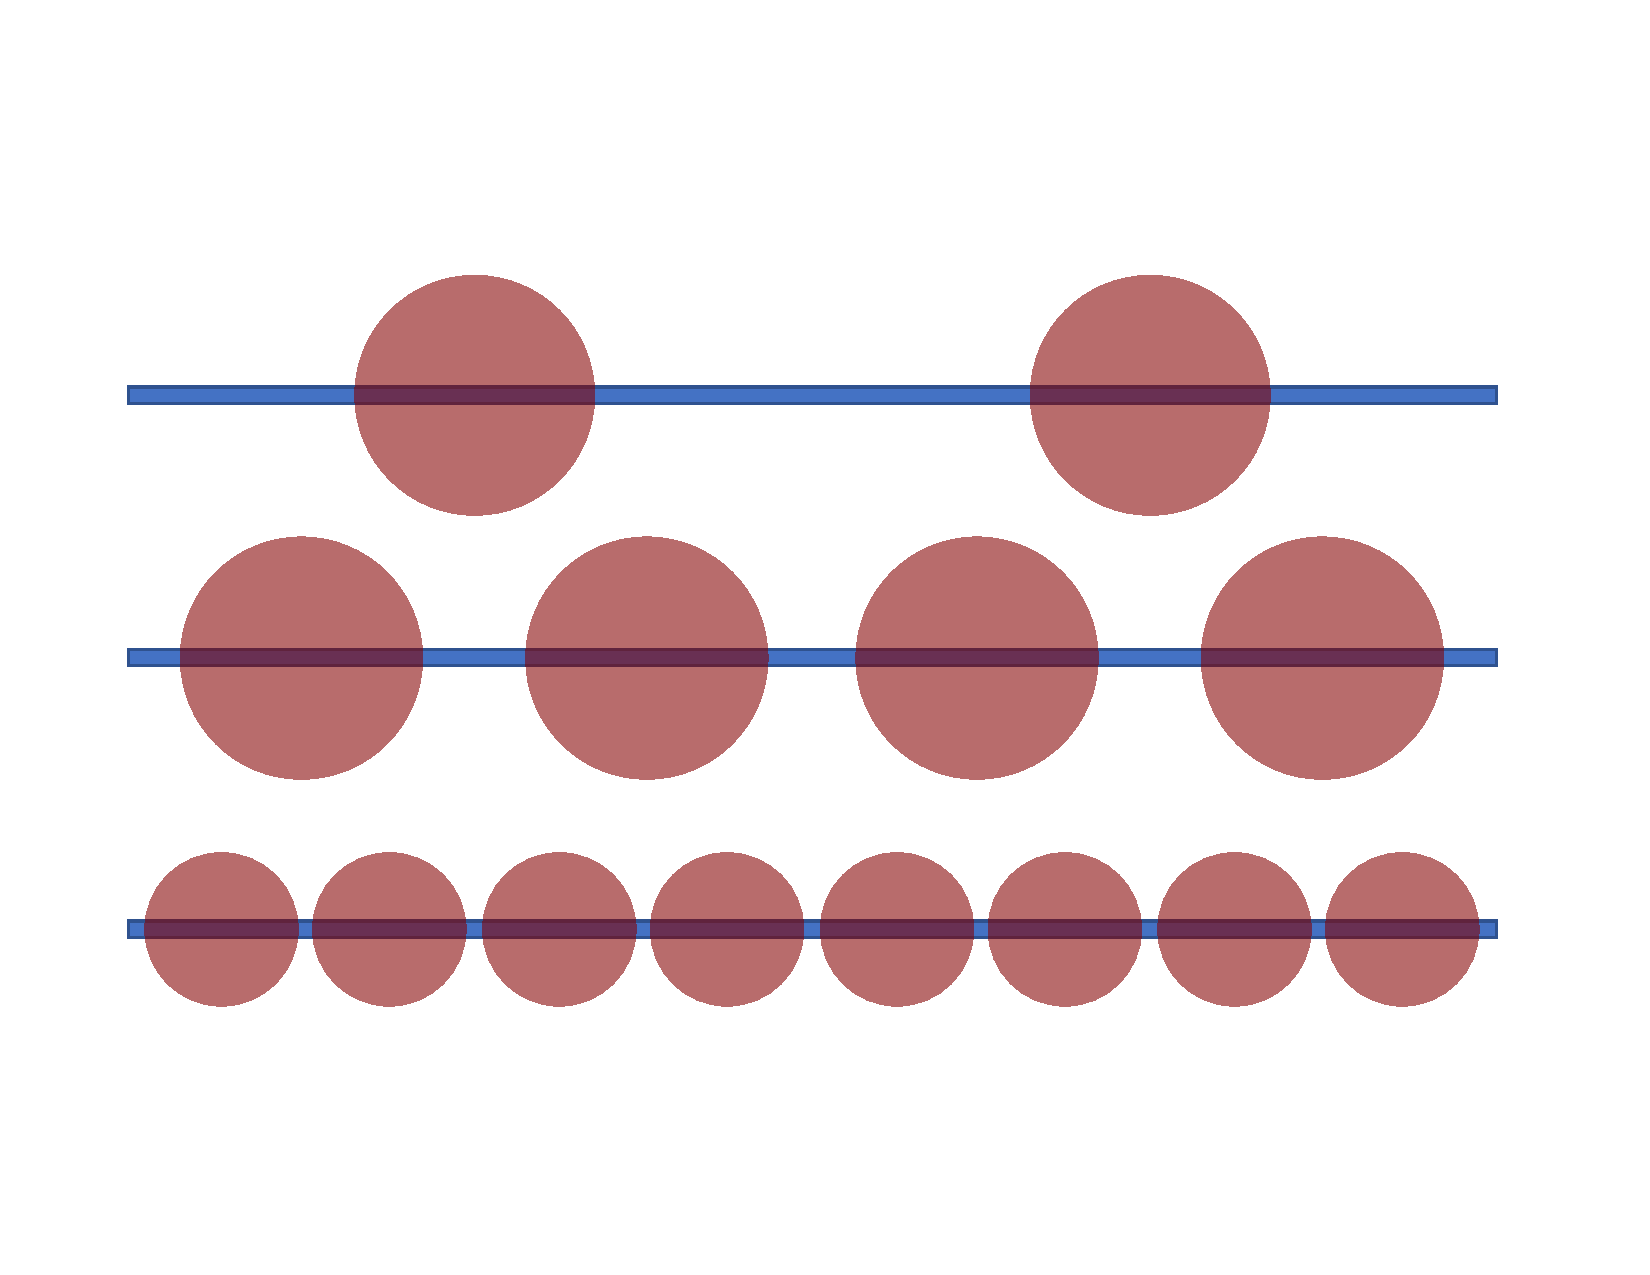
\includegraphics[trim={2.0cm 3.5cm 2.0cm 4.5cm},clip,angle = 0,width=3.0in]{propsize}
    \caption{Visual depiction of optimal rotor diameters relative to wingspan for the 45 m/s cruise case. For more than eight propellers, the blades are effectively tip-to-tip across the span.}
    \label{f:propsize}
\end{figure}


\subsection{Noise Constraint Sweep}

\label{sec:noise}

For our second set of results, we explore noise constraints less than the maximum permissible for the aircraft (76 dBa) at a 100 mph cruise speed (from the first set of results). Since the first solutions converge to approximately 70 dBa, we reduced the allowable noise constraint to three fourths and then half the perceived SPL (65 and 60 dBa) and observed a diverging trend of the curve.  We included a 63 dBa constraint to more accurately show the trend. Noise is a key element for new aircraft to be of value~\cite{Moore:2014aa}, especially when considering the type of environment in which these aircraft might fly. The noise we report for this conceptual design study is calculated as the max SPL in takeoff at 50 feet relative to a ground observer and in line with the aircraft center axis. According to the most recent FAA noise levels advisory for this weight of aircraft\footnote{FAA Advisory Circulars \href{https://www.faa.gov/airports/resources/advisory\_circulars/index.cfm/go/document.information/documentNumber/36-1H}{https://www.faa.gov/airports/resources/advisory\_circulars}, accessed 4/11/19}, the maximum allowable SPL is 76 dB(a). According to the Tecnam aircraft manual\footref{p2006t}, the maximum SPL for the aircraft, in accordance with the International Civil Aviation Organization, is 67.07 dB(a). While we rely on the BPM noise code as an approximation, the maximum takeoff noise for the two propeller case does fall within the correct range at about 67.6 dBa for the 22 m/s cruise speed case increasing to 69.3 dBa for the 67 m/s cruise speed case.


\Cref{f:takeoff_noise} shows the effect of the propeller noise constraint on the takeoff distance with varying numbers of propellers. For all of the cases tested, as noise decreased, there was a divergent increase in the takeoff distance. Focusing on the best case with respect to the constraints, eight propeller case, there was only a 15\% increase in the takeoff distance between propeller noise constraints of less than 76 (converged to 71) dBa and 65 dBa, which translates to about 3/4 of the perceived noise level. However, for very strenuous noise constraints, the trend becomes divergent with an additional 50\% increase increase in takeoff distance between noise constraints of 65 and 60 dBa.

\begin{figure}[htbp]
    \centering
    \includegraphics[width=3.0in]{takeoff_speed_db}:
    \caption{Noise constraint effects on optimal takeoff distance with a fixed 45 m/s cruise speed constraint. Decreasing the propeller noise constraint significantly increases takeoff distance. Less-than symbol indicates noise constraint was not active }
    \label{f:takeoff_noise}
\end{figure}

Moving from the 8 propeller to 16 propeller cases, it would appear that an exponential trend in takeoff distance would continue with 32 propellers. However, the opposite is true due to the propellers' design and operating condition. As discussed in \cref{sec:prop_noise}, the noise production is non-intuitive with varying number of propellers, geometry, and number of blades. For these analyses, the number of blades was optimized by first including number of blades as a continuous design variable since the BEM calculation does not require an integer number of blades. Then, with a converged solution, we round the number of blades to an integer value and re-optimize.  The number of blades for the 2, 4, 8, 16, and 32 propeller cases always came to 2, 2, 2, 4, and 5 blades respectively, except for the 60 dBa case where 16 propellers converged to 3 blades.  The full propeller design and operating conditions need to be included to get an adequately accurate prediction on the noise produced.

\subsubsection{Noise Constrained Thrust}


While the optimal propeller diameter and solidity remain relatively constant for a given number of propellers under the varying noise constraint, the tip speed for more propellers decreases sharply. To achieve a similar SPL between many high solidity propellers and a few lower solidity propellers, the tip speed of the greater number of propellers must be significantly decreased. From the thrust coefficient equation $T = C_T \rho n^2 D^4$, with a relatively constant coefficient of thrust $C_T$, air density $\rho$, and diameter $D$, but changing rotation rate $n$, the generated thrust is decreased in an $n^2$ manner due to decreased tip speed. The effects of this can be seen in \cref{fig:Climb_Thrust2Weight_db} with the greater number of propellers experiencing a much greater penalty on thrust to weight with decreasing noise constraint. However, even down to a noise constraint of 63 dBa, the eight propeller takeoff distance is still below 100 m.

\vspace{11pt}

\begin{figure}[H]
    \centering
    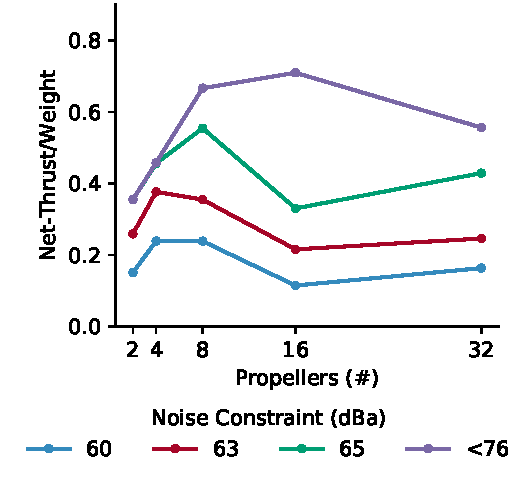
\includegraphics[trim={0.3cm 0.25cm 0.0cm 0.25cm},clip,width=3.0in]{Climb_NetThrust2Weight_db}
    \caption{Climb net thrust to weight with noise constraint effects, 45m/s cruise. Compare \cref{fig:Climb_Thrust2Weight}. Total climb thrust in excess of 70\% of the aircraft weight when the constraints on cruise speed are inactive.}
    \vspace{-10pt}
    \label{fig:Climb_Thrust2Weight_db}
\end{figure}

\subsubsection{Noise Constrained Lift Coefficient}


With the decrease in available thrust due to the tip speed constraint, the propeller wake velocity is also decreased. This decreases the dynamic pressure relative to a case with a higher blown velocity, and in turn, decreases the wing lift coefficient. As seen in \cref{fig:CL_TO_db} for the eight propeller case, the lift coefficient is decreased from 5.0 at the 76 dBa constraint level to 3.5 at the 63 dBa constraint level. With decreased available thrust and decreased wing lift coefficient, it takes longer to accelerate the same aircraft mass to a higher takeoff speed and still clear the 50 ft obstacle.

\vspace{11pt}

\begin{figure}[htbp]
    \centering
    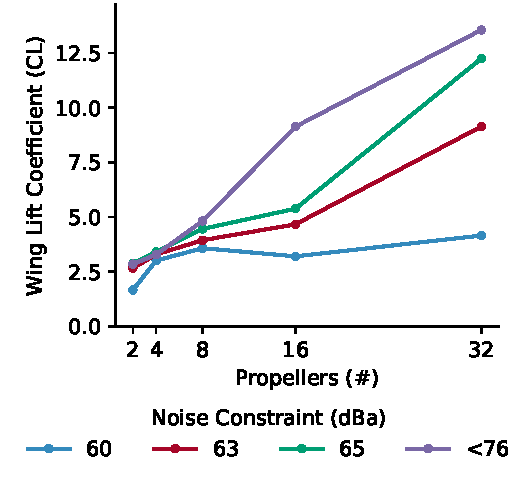
\includegraphics[trim={0.3cm 0.25cm 0.0cm 0.25cm},clip,width=3.0in]{CL_climb_db}
    \caption{Wing lift coefficient in the climb state.  Compare \cref{fig:CL_climb}. Noise constraints significantly decrease the ability of more propellers to produce excess dynamic pressure and in turn augmented lift coefficients.}
    \label{fig:CL_TO_db}
\end{figure}


%%%%%%%%%%%%%%%%%%%%
%%  END RESULTS
%%  START CONCLUSIONS
%%%%%%%%%%%%%%%%%%%%

\section{Conclusions}

\label{Conclusions}

In this study, we explored how continuously powered distributed electric propulsion on a Tecnam p2006t airframe could be used as an immediate potential alternative to current urban air transport concepts. In this conceptual design study, we found that a fully blown wing with 16 propellers could reduce the takeoff distance by over 50\% when compared to the optimal 2 propeller case. This resulted in a conceptual minimum takeoff distance of 20.5 meters to clear a 50 ft (15.24 m) obstacle. We found that when decreasing the allowable noise to 60 dBa, the fully blown 8 propeller case performed the best with a 43\% reduction in takeoff distance compared to the optimal 2 propeller case at the same noise constraint. The increase in takeoff distance due to noise constraints was divergent with relatively little effect until the noise-performance tradeoffs become significant at levels below 65 dBa for all cases tested. For the 8 propeller case at the 65 dBa constraint (70\% of the perceived sound pressure level) there was only a 15\% increase in the takeoff distance. This case yielded a total conceptual takeoff distance of approximately 37 m. Further reducing allowable noise to a 60 dBa constraint (50\% perceived noise reduction) resulted in an additional 2.4x increase in takeoff distance for the 8 propeller case.

We concluded that based on the results of this study, a distributed electric propulsion short takeoff and landing fixed wing aircraft may be a candidate for the on demand mobility (ODM) urban air transport problem and warrants future work in the area. The retrofit propulsion system in this study conceptually enabled the existing Tecnam p2006t to achieve conceptual takeoff distances which would open thousands of potential options for urban air taxi runways. When cruise speed and noise constraints are also included, the fully blown DEP system was still able to outperform the more traditional 2 propeller system for the short range requirement modeled and still achieve a takeoff distance of less than 100 meters.

The main areas of future work critical to this study are in the design fidelity and the certification requirements. On the design side, work could include more design freedom to completely change an aircraft configuration for a given mission. Some possibilities include modeling propeller design that varies along the wingspan as well as including propellers above or below the chord line to further influence the lift distribution and system efficiency. Optionally powered and overlapping units, as well as including aircraft constraints on things such as brakes for landing, fuselage structure for increased wing loading, stability, control, and full wing redesign could be included. The noise of the electric motors, lifting surfaces, and control surfaces, could be added into the noise model. The second order motor model including heat transfer could be included as well as a time-dependent battery model. Additionally, one might model the landing portion of the flight including a final landing approach suggested by Patterson et al.~\cite{Patterson:2017aa}, expand on the landing as modeled by Courtin et al.~\cite{Courtin:2018aa}, and model the optimal flight path similar to work by Hwang~\cite{Hwang:2018aa}.

On the certification side, which is a critical component to the potential implementation of this concept, there is significant work that would need to be done to access the safety, flight requirements, and potential changes to stall regulations similar to those also suggested by Patterson~\cite{Patterson:2017aa} as well as required total field length when a balanced field length is so short. Other areas may address safety requirements with multiple partially independent propulsion units, urban gust and building wind factors, and required infrastructure.

\section{Code}


The final code and data used to produce this work will be available on the BYU FLOW Lab website\footnote{FLOW Lab \href{http://flow.byu.edu}{http://flow.byu.edu}} following a six month embargo period.


\section*{Acknowledgments}

The authors gratefully acknowledge support from The Connectivity Lab at Facebook.

\newpage

\bibliography{refs}
\bibliographystyle{aiaa}
\end{document}
